\documentclass[aspectratio=169]{beamer}
\usetheme{metropolis}           % Use metropolis theme
\setbeamercolor{background canvas}{bg=white}
\title{\phantom{a}
\\
An Introduction to Explainable AI with
\\ SHapley Additive exPlanations (SHAP)
\\
\phantom{a}
}

\usepackage[linesnumbered,ruled,vlined]{algorithm2e}

\setbeamersize{text margin left=3mm,text margin right=3mm} 

\date[conf-name]{}

\usepackage{hyperref}
\setbeamertemplate{frametitle}{%
    \nointerlineskip%
    \begin{beamercolorbox}[wd=\paperwidth,ht=2.5ex,dp=1ex]{frametitle}
        \hspace*{1ex}\insertframetitle%
    \end{beamercolorbox}%
}

\usepackage{acronym}

\appto\citesetup{\tiny}

\definecolor{processblue}{RGB}{0,133,202}
\definecolor{brightorange}{RGB}{255,94,0}
\titlegraphic{\vspace{1.3cm}\flushright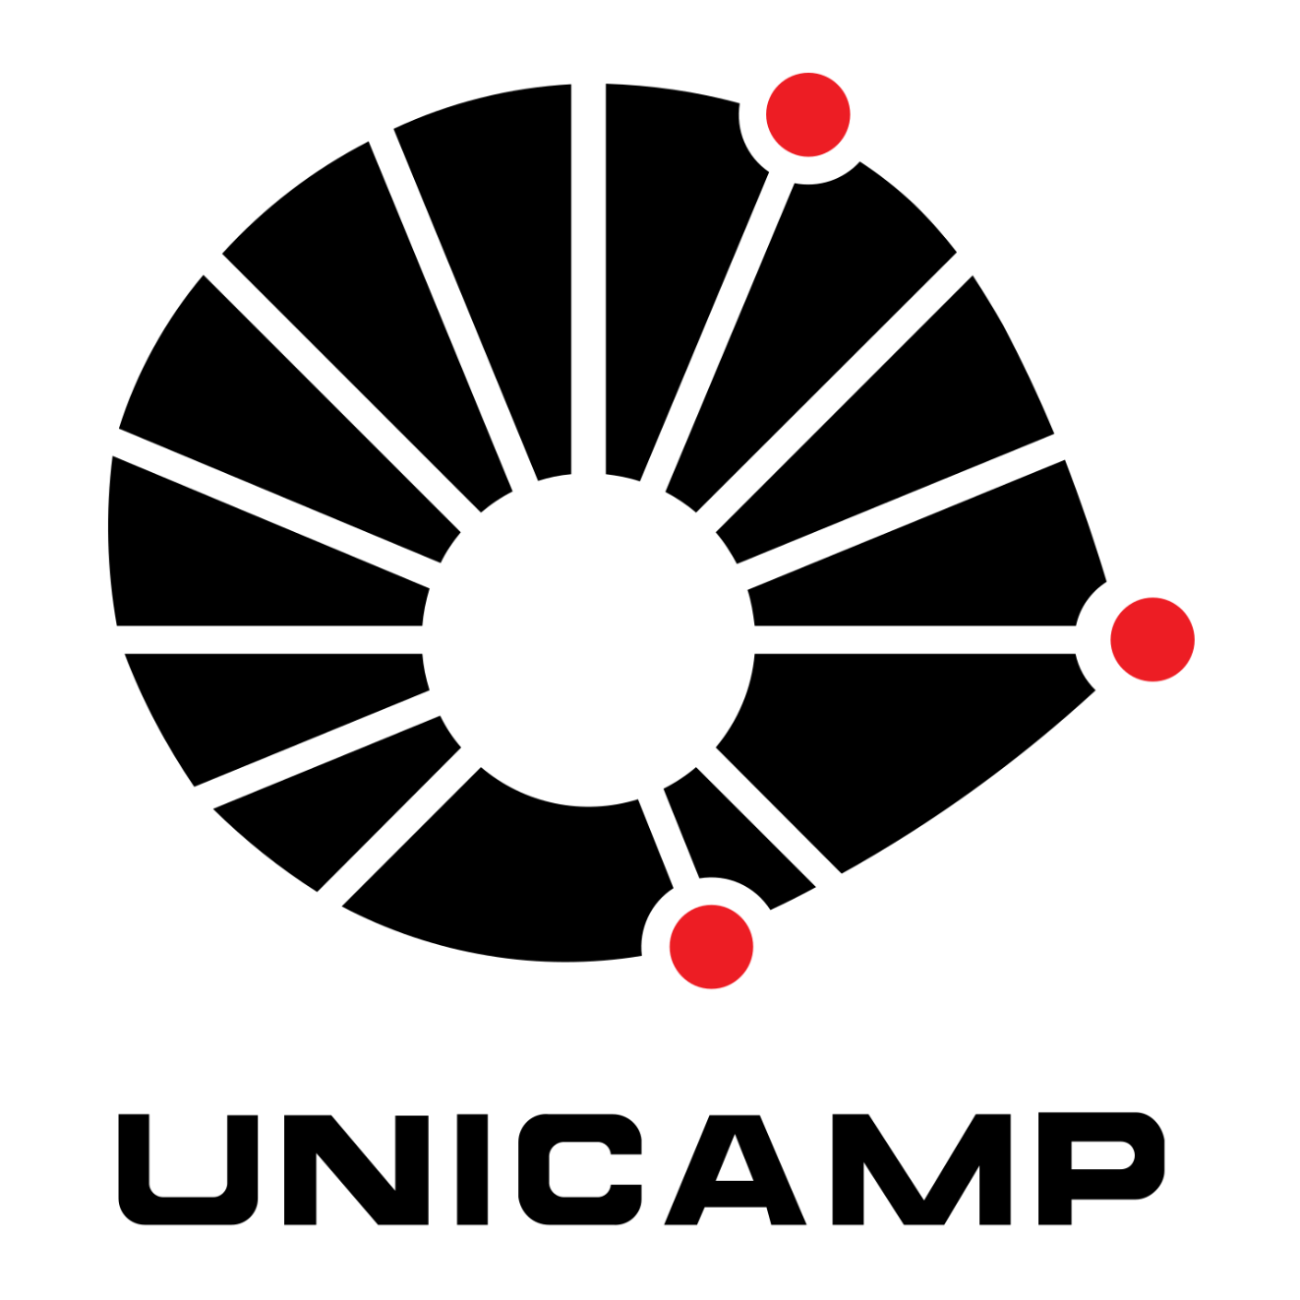
\includegraphics[width=2cm,height=2cm]{figs/UNICAMP.png}\\
\vspace{0.8cm}\flushright
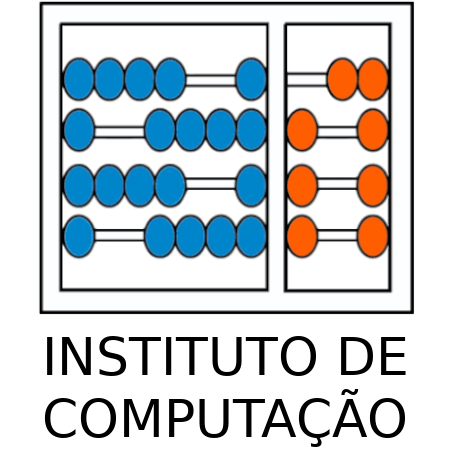
\includegraphics[width=2cm,height=2cm]{figs/IC.png}

\includegraphics[width=2cm,height=2cm]{figs/RECOD.png}
}
\newcommand{\question}[1]{\vspace{\fill}\begin{center}\textbf{#1}\end{center}}
\setbeamercolor{frametitle}{bg=processblue}%, fg=brightorange}
\setbeamercolor{title separator}{fg=brightorange, bg=brightorange}
\setbeamercolor{progress bar}{fg=brightorange, bg=brightorange}
\makeatletter
\setlength{\metropolis@titleseparator@linewidth}{1pt}
\setlength{\metropolis@progressonsectionpage@linewidth}{1pt}
\setlength{\metropolis@progressinheadfoot@linewidth}{1pt}
\AtBeginSubsection{\frame{\subsectionpage}}


\author{
João Victor P. B. Avanzini \\
Advisor: Marcos M. Raimundo \\
RECOD.AI - Institute of Computing - Unicamp \\
Nov 6, 2023 - Campinas - Brazil}

\usepackage{graphicx}
\usepackage{caption}
\usepackage{subcaption}
\usepackage{multirow}

\usepackage{tikz}
\usetikzlibrary{arrows,positioning,calc}
\usetikzlibrary{fit,backgrounds}
\usetikzlibrary{patterns}

\usepackage{pgfplots}

\usepackage{listings}

\pgfplotsset{
  compat=1.3,
  width=4.5cm,
  height=4cm}
  
\tikzstyle{line} = [draw, -latex']

\renewcommand\vec{\mathbf}

\DeclareUnicodeCharacter{2212}{-}

\begin{document}

%\input{figures}

\maketitle


\begin{acronym}
  \acrodef{AD}{Autonomic Dysreflexia}
  \acrodef{MIMIC}{Medical Information Mart for Intensive Care}
  \acrodef{AAMI}{Association for the Advancement of Medical Instrumentation}
  \acrodef{BP}{Blood Pressure}
  \acrodef{SBP}{Systolic Blood Pressure}
  \acrodef{DBP}{Diastolic Blood Pressure}
  \acrodef{ABP}{Arterial Blood Pressure}
  \acrodef{MAP}{Mean Arterial Pressure}
  \acrodef{PPG}{Photoplethysmogram}
  \acrodef{PIR}{Photoplethysmogram Intensity Ratio}
  \acrodef{PTT}{Pulse Transit Time}
  \acrodef{ECG}{Electrocardiogram}
  \acrodef{mmHg}{Millimetre of mercury}
  \acrodef{AI}{Artificial Intelligence}
  \acrodef{ML}{Machine Learning}
  \acrodef{DL}{Deep Learning}
  \acrodef{DNN}{Deep Neural Network}
  \acrodef{ResNet}{Residual Neural Network}
  \acrodef{LSTM}{Long short-term memory}
  \acrodef{ANN}{Artificial Neural Network}
  \acrodef{NNOE}{Output-Error Neural networks}
  \acrodef{MAE}{Mean Absolute Error}
  \acrodef{AAE}{Average Absolute Error}
  \acrodef{MSE}{Mean Square Error}
  \acrodef{RMSE}{Root Mean Square Error}
  \acrodef{RNN}{Recurrent Neural Network}
  \acrodef{LOSO}{Leave-One-Subject-Out}
  \acrodef{XAI}{Explainable Artificial Intelligence}
  \acrodef{LIME}{Local interpretable model-agnostic explanations}
  \acrodef{SHAP}{SHapley Additive exPlanations}
  \acrodef{PDP}{Partial Dependence Plot}
  \acrodef{LRP}{Layer-wise Relevance Propagation}
  \acrodef{SA}{Sensitivity Analysis}
  % Add more acronyms as needed
\end{acronym}

\section{Schedule}

\begin{frame}{Schedule}

    \begin{itemize}
        \item Introduction to \ac{SHAP}
        \item \ac{SHAP} Overview
        \item Core Concept
        \item Installation
        \item Understanding Explainability
        \item Plots
        \item Project Examples
        \item Reference
        \item Benchmarks
        \item Release Notes
        \item Thank you for exploring \ac{SHAP}!
    \end{itemize}

\end{frame}


\begin{frame}{\ac{SHAP}}
    \begin{figure}[htbp]
        \centering
        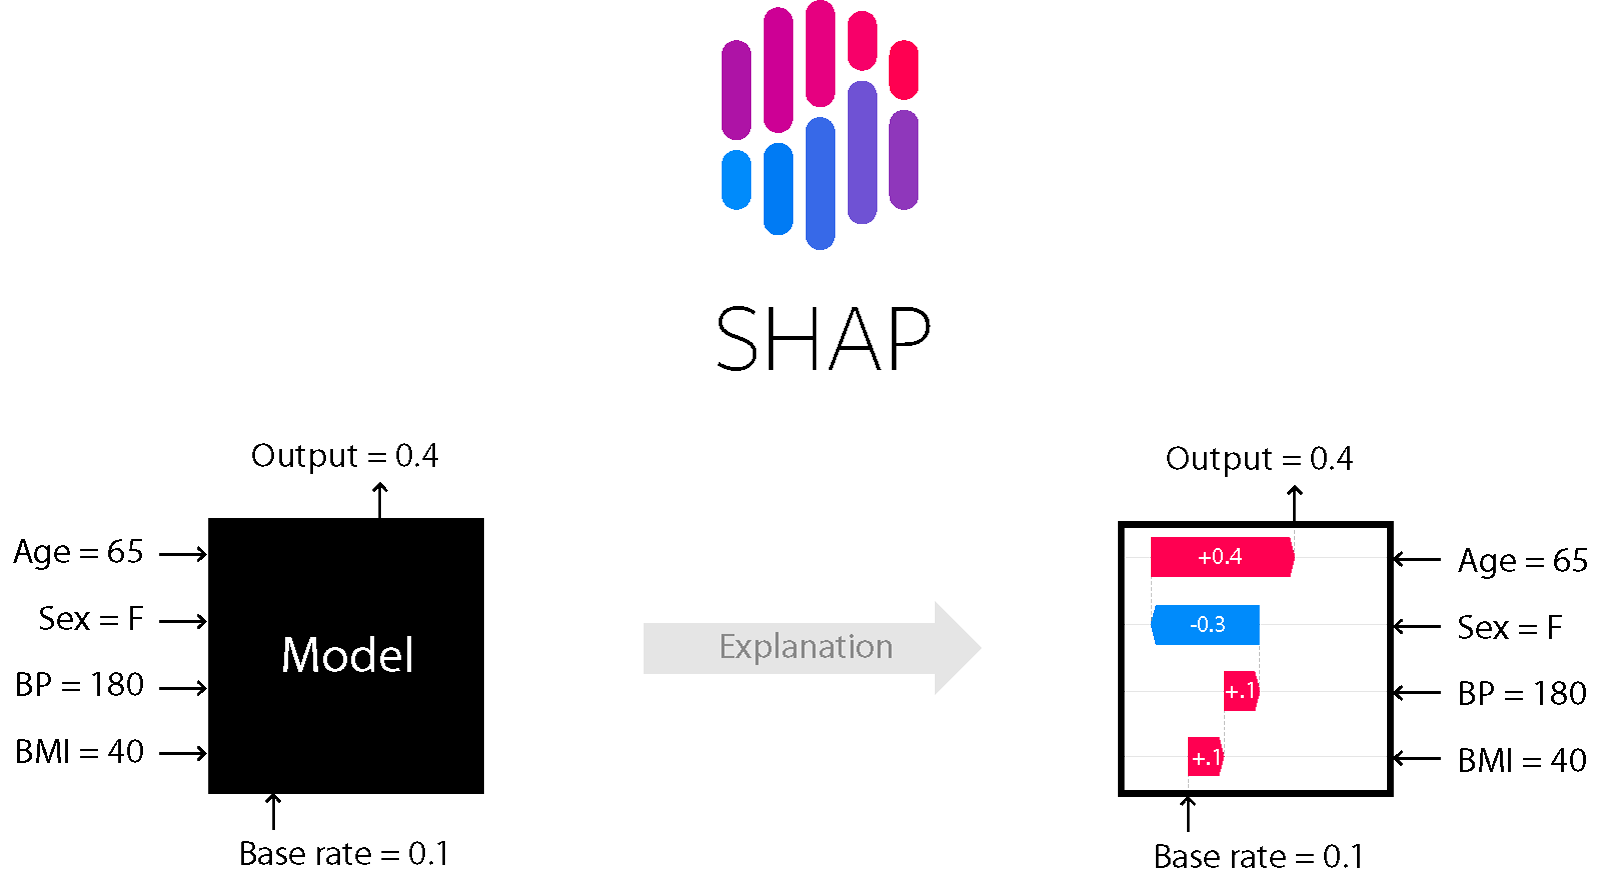
\includegraphics[width=0.7\textwidth]{figs/shap/shap_header.png}
        \caption{\ac{SHAP} logo}
        \label{fig:shap}
    \end{figure}
\end{frame}

\section{Introduction to \ac{SHAP}}

\begin{frame}{Introduction to \ac{SHAP}}
    \ac{SHAP} is a game-theoretic approach to \textbf{explain the output of any \ac{ML} model}. It connects \textbf{optimal credit allocation} with \textbf{local explanations} using the classic \textbf{Shapley values} from game theory and their related extensions.
\end{frame}

\begin{frame}{Links - Introduction to \ac{SHAP}}
    \begin{itemize}
        \item \textbf{Documentation:} \url{shap.readthedocs.io}
        \item \textbf{GitHub:} \url{github.com/shap/shap}
    \end{itemize}
    
\end{frame}

\section{\ac{SHAP} Overview}

\begin{frame}{\ac{SHAP} Overview}
    \begin{itemize}
        \item The Shapley value is a solution concept used in game theory that involves fairly distributing both gains and costs to several actors working in a coalition.
    
        \item Game theory is when two or more players or factors are involved in a strategy to achieve a desired outcome or payoff.
    
        \item The Shapley value applies primarily in situations when the contributions of each actor are unequal, but each player works in cooperation with each other to obtain the gain or payoff.

        \item The Shapley value ensures each actor gains as much or more as they would have from acting independently. The value obtained is critical because otherwise there is no incentive for actors to collaborate. The Shapley value–named after Lloyd Shapley --- has many applications, including business, \ac{ML}, and online marketing.
        
    \end{itemize}
\end{frame}

\begin{frame}{Outline - \ac{SHAP} Overview}
    \begin{itemize}
        \item Explaining a linear regression model
        \item Explaining a generalized additive regression model
        \item Explaining a non-additive boosted tree model
        \item Explaining a linear logistic regression model
        \item Explaining a non-additive boosted tree logistic regression model
        \item Dealing with correlated input features
        \item Explaining a transformers NLP model
    \end{itemize}
\end{frame}


\begin{frame}{Explaining quantitative measures of fairness - \ac{SHAP} Overview}
    Quantitative fairness metrics seek to bring mathematical precision to the definition of fairness in \ac{ML}. Definitions of fairness however are deeply rooted in human ethical principles, and so on value judgements that often depend critically on the context in which a \ac{ML} model is being used. This practical dependence on value judgments manifests itself in the mathematics of quantitative fairness measures as a set of trade-offs between sometimes mutually incompatible definitions of fairness. Since fairness relies on context-dependent value judgments it is dangerous to treat quantitative fairness metrics as opaque black-box measures of fairness, since doing so may obscure important value judgment choices. Provided by \ac{SHAP} documentation.
\end{frame}

\section{Core Concept}

\begin{frame}{Game theory - Core Concept}

This slide presents the Shapley value, which is one of the two most important single-valued solution concepts for coalitional games. It assigns to every coalitional game an imputation, which represents the payoff that each player can expect to obtain from participating in the game. The Shapley value is defined by an axiomatic approach: it is the unique solution concept that satisfies the efficiency, symmetry, null player, and additivity properties. An explicit formula is provided for the Shapley value of a coalitional game, as a linear function of the worths of the various coalitions. A second characterization, due to Peyton Young, involves a marginality property that replaces the additivity and null player properties. Maschler et al. \cite{cup_2013}
    
\end{frame}

\begin{frame}{Game theory - Core Concept}

The Shapley value of a convex game turns out to be an element of the core of the game, which implies in particular that the core of a convex game is nonempty. Similar to the core, the Shapley value is consistent: it satisfies a reduced game property, with respect to the Hart–Mas-Colell definition of the reduced game.

When applied to simple games, the Shapley value is known as the Shapley–Shubik power index and it is widely used in political science as a measure of the power distribution in committees. Maschler et al. \cite{cup_2013}
    
\end{frame}

\begin{frame}{Game theory - Core Concept}

\begin{figure}
    \centering
    
\includegraphics[width=0.35\textwidth]{figs/shap/game_theory.jpeg}
    \caption{The book of Cambridge University Press \cite{cup_2013}}
    \label{fig:game-theory}
\end{figure}
    
\end{frame}

\begin{frame}{Optimal Credit Location - Core Concept}
    The Kelly Criterion for Optimal Credit Allocation is discussed in the Journal of Risk and Financial Management by Son Tran and Peter Verhoeven \cite{Tran2021}. The authors explore the obstacles in performance assessment when converting a borrower's chance of default into labeled groups and give suggestions on estimating a borrower's risk of default. The paper additionally demonstrates the significance of a credit allocation system capable of dispersing parts of a loan among many lenders concurrently. According to the authors, seeing credit risk modeling as an allocation problem will lead to a better understanding of how the work may be done successfully and efficiently in practice. The paper concludes with research recommendations, such as investigating the basis of the Kelly criterion's outperformance and defining the technical infrastructure necessary for a credit allocation system.
\end{frame}

\begin{frame}{Local Explanations - Core Concept}
    Local explanations are a form of interpretability tool that may assist users in understanding how a machine learning model arrived at a certain prediction for a given input or sample. Local explanations may be constructed in the context of tree-based models by assessing the contribution of each feature or variable to the final forecast for a particular input. Lundberg et al. \cite{Lundberg2020}

\end{frame}

\begin{frame}{Local Explanations - Core Concept}
    Local explanations can help with model debugging, feature engineering, and recognizing any biases or flaws in the model. They may also help address transparency requirements in regulated fields such as healthcare and finance, where understanding how a model arrived at a given choice is critical. Lundberg et al. \cite{Lundberg2020}
\end{frame}

\begin{frame}{Local Explanation - Core Concept}
    \begin{figure}[htbp]
        \centering
        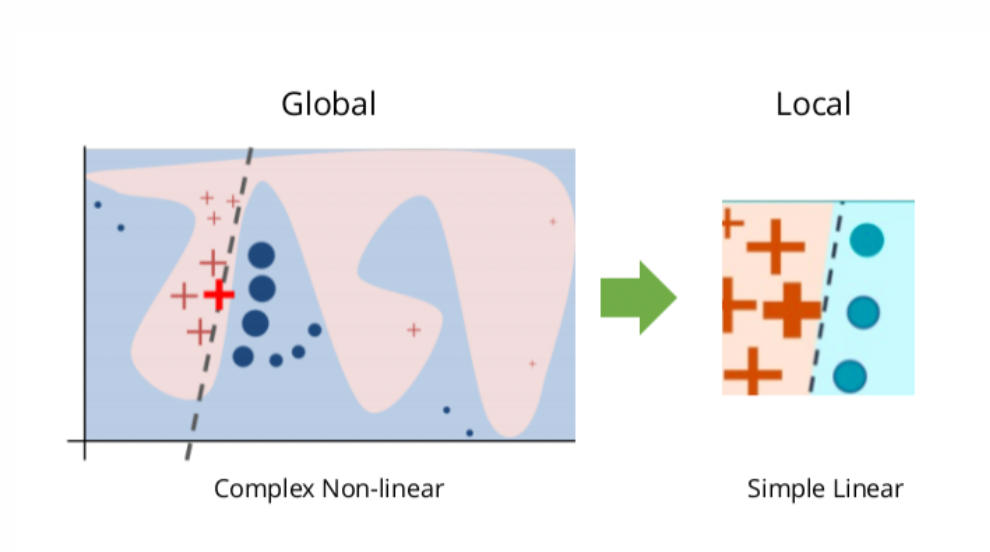
\includegraphics[width=0.7\textwidth]{figs/xai/local_explanation.png}
        \caption{Cohort and local approximation of an example for interpretability employing a linear model inside a region of interest. Image by c3.ai}
        \label{fig:local-explanation}
    \end{figure}
\end{frame}

\section{Installation}

\begin{frame}[fragile]{Extremely easy method - Installation}

\begin{lstlisting}[language=bash]
# Using pip
pip install shap

# Using conda
conda install -c conda-forge shap
\end{lstlisting}
    
\end{frame}

\section{Understanding Explainability}

\begin{frame}{Understanding AI with Shapley values - Understanding Explainability}
    \begin{enumerate}
        \item Introduction to Explainability
        \item Shapley Values in Explainability
        \item Practical Application
        \item Cautions in Model Interpretation
        \item Quantitative Measures of Fairness
    \end{enumerate}
\end{frame}

\begin{frame}{Introduction to Explainability - Understanding Explainability}
    \begin{figure}[htbp]
        \centering
        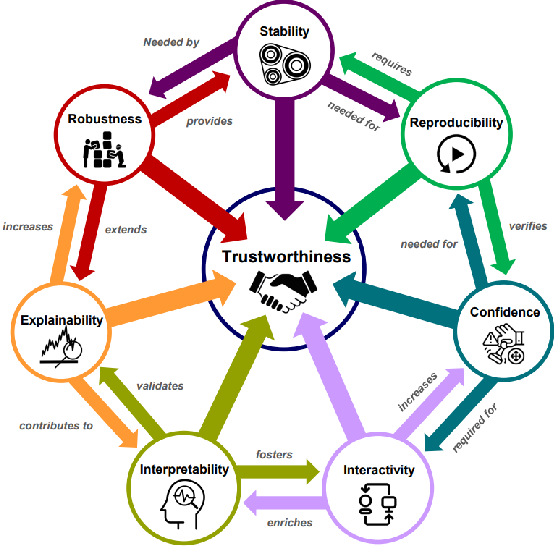
\includegraphics[width=0.45\textwidth]{figs/xai/xai-cicle.png}
        \caption{Knowledge graph relating all the purposes of explainability methods, by Rojat et al. \cite{DBLP:journals/corr/abs-2104-00950}}
        \label{fig:xai-circle}
    \end{figure}
\end{frame}

\begin{frame}{Introduction to Explainability - Understanding Explainability}

Rojat et al. \cite{DBLP:journals/corr/abs-2104-00950} show that explainability is important for many reasons:

    \begin{itemize}
        \item \textbf{Transparency}:
        Explainability enables insight into how \ac{AI} models make decisions, which is critical to establishing trust and responsibility.
        \item \textbf{Interpretability}:
        Explainability improves the interpretability of \ac{AI} models, which is critical in fields where human specialists must comprehend the logic behind the model's judgments. In healthcare, for example, clinicians must comprehend why a model recommends a specific treatment.
        \item \textbf{Robustness}:
        By detecting any biases or flaws in the model decision-making process, explainability could assist in increasing the robustness of \ac{AI} models. This can assist in keeping the model from making mistakes or harming itself.
        \item \textbf{Compliance}:
        Legal and regulatory requirements for explainability exist in various fields, such as banking and healthcare. To comply with these requirements, \ac{AI} models must be able to explain their conclusions.
    \end{itemize}

\end{frame}

\begin{frame}{Shapley Values in Explainability - Understanding Explainability}

The Shapley value is the only explanation method with a solid theory. The axioms – efficiency, symmetry, dummy, additivity – explain a reasonable foundation. Molnar et al. \cite{molnar2022}

\end{frame}

\begin{frame}{Practical Application - Understanding Explainability}

    \begin{figure}[htbp]
        \centering
        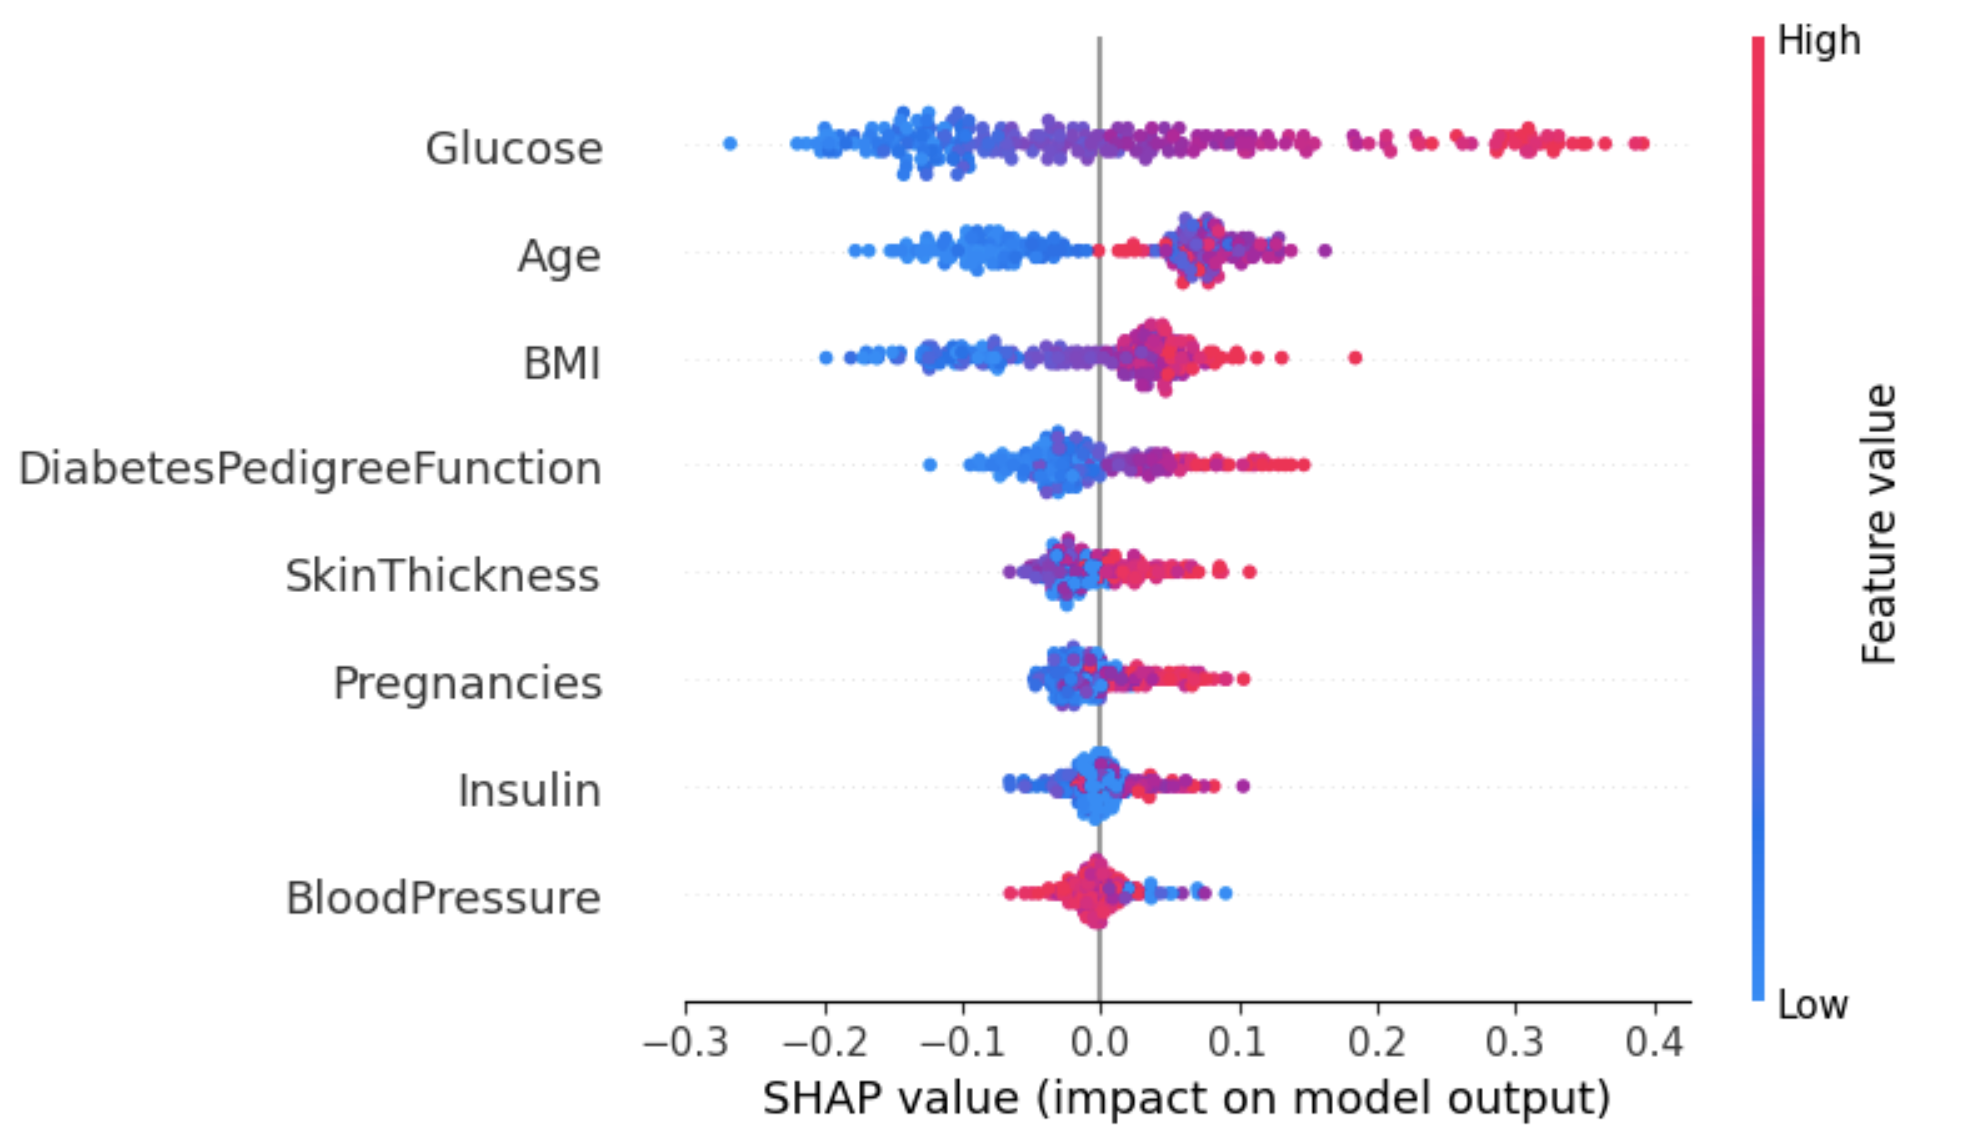
\includegraphics[width=0.8\textwidth]{figs/shap/Summary_Plot_deep_dive_on_label_diabete.png}
        \caption{Summary plot for explain diabetes. Image by Datacamp.com: \cite{datacamp_tutorial}}
        \label{fig:explain-diabetes}
    \end{figure}
\end{frame}

\begin{frame}{Practical Application - Understanding Explainability}

    \begin{itemize}
        \item Y-axis represents the features ranked by their average absolute \ac{SHAP} values.
        \item X-axis represents \ac{SHAP} values. Positive values for a given feature push the model’s prediction closer to the label being examined (label=1). In contrast, negative values push towards the opposite class (label=0)
        \item An individual with a high glucose (red dots) level is likely to be diagnosed with diabetes (positive outcome), while a low glucose level leads to not being diagnosed with diabetes.
        \item Similarly, aging patients are more likely to be diagnosed with diabetes. However, the model seems uncertain about the diagnosis for younger patients.
    \end{itemize}

    Text by Datacamp.com: \cite{datacamp_tutorial}
\end{frame}

\begin{frame}{Cautions in Model Interpretation - Understanding Explainability}

It's difficult to understand the \ac{SHAP} graphics, but patience is required.
    
\end{frame}

\begin{frame}{Quantitative Measures of Fairness - Understanding Explainability}
     We can decompose measures of fairness and allocate responsibility for any observed disparity among each of the model’s input features. Explaining these quantitative fairness metrics can reduce the concerning tendency to rely on them as opaque standards of fairness, and instead promote their informed use as tools for understanding how model behavior differs between groups. Provided by \ac{SHAP} documentation \cite{shap_docs_fairness}.
\end{frame}

\begin{frame}{Quantitative Measures of Fairness - Understanding Explainability}
     Quantitative fairness metrics seek to bring mathematical precision to the definition of fairness in \ac{ML} Kearns et al. \cite{10.5555/3379082}. Definitions of fairness however are deeply rooted in human ethical principles, and so on value judgements that often depend critically on the context in which a \ac{ML} model is being used. This practical dependence on value judgments manifests itself in the mathematics of quantitative fairness measures as a set of trade-offs between sometimes mutually incompatible definitions of fairness Kleinberg et al. \cite{DBLP:journals/corr/KleinbergMR16}. Since fairness relies on context-dependent value judgments, it is dangerous to treat quantitative fairness metrics as opaque black-box measures of fairness, since doing so may obscure important value judgment choices. Provided by \ac{SHAP} documentation \cite{shap_docs_fairness}.
\end{frame}

\section{Plots}

\begin{frame}{Types - Plots}
    \begin{itemize}
        \item \textbf{Bar}
        \item \textbf{Beeswarm}
        \item \textbf{Decision}
        \item \textbf{HeatMap}
        \item \textbf{Image}
        \item \textbf{Scatter}
        \item \textbf{Text}
        \item \textbf{Violin}
        \item \textbf{WaterFall}
    \end{itemize}   
\end{frame}

\begin{frame}{Global bar - Plots}
Passing a matrix of \ac{SHAP} values to the bar plot function creates a global feature importance plot, where the global importance of each feature is taken to be the mean absolute value for that feature over all the given samples.
    \begin{figure}[htbp]
        \centering
        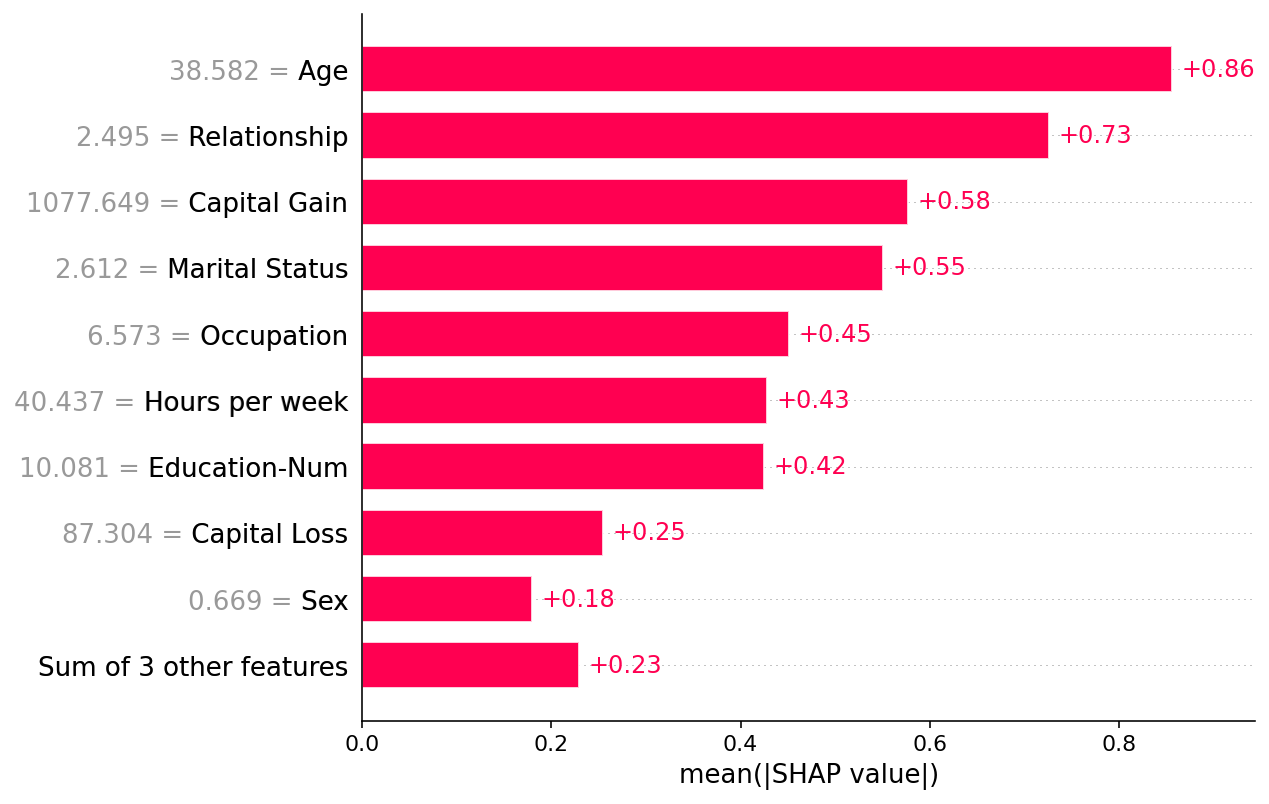
\includegraphics[width=0.55\textwidth]{figs/shap/plots/bar/example_notebooks_api_examples_plots_bar_3_0.png}
        \caption{Global bar plot}
        \label{fig:global-bar}
    \end{figure}
\end{frame}

\begin{frame}{Local bar - Plots}
Passing a row of \ac{SHAP} values to the bar plot function creates a local feature importance plot, where the bars are the \ac{SHAP} values for each feature. Note that the feature values are colored gray to the left of the feature names.
    \begin{figure}[htbp]
        \centering
        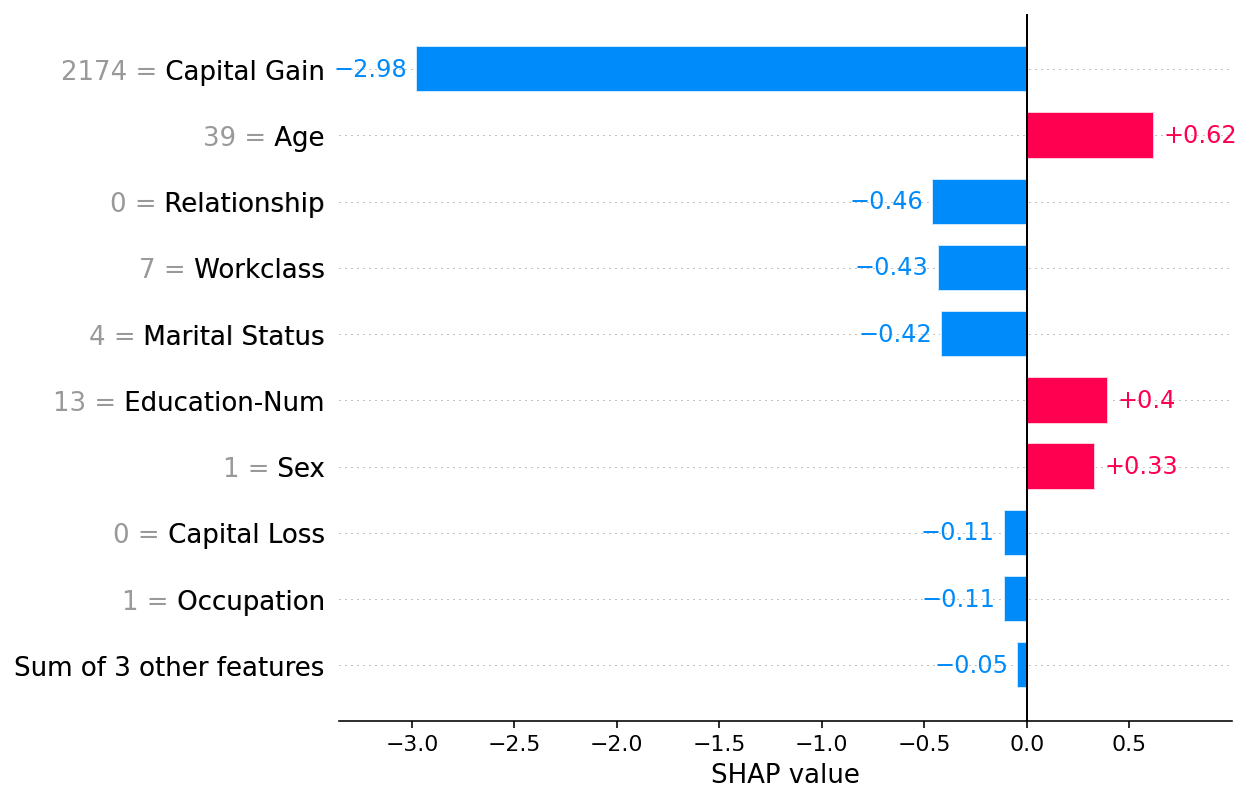
\includegraphics[width=0.55\textwidth]{figs/shap/plots/bar/example_notebooks_api_examples_plots_bar_7_0.png}
        \caption{Local bar plot}
        \label{fig:Local-bar}
    \end{figure}
\end{frame}

\begin{frame}{Global cohort bar plot - Plots}
Passing a dictionary of Explanation objects will create a multiple-bar plot with one bar type for each of the cohorts represented by the explanation objects. Below we use this to plot a global summary of feature importance separately for men and women.
    \begin{figure}[htbp]
        \centering
        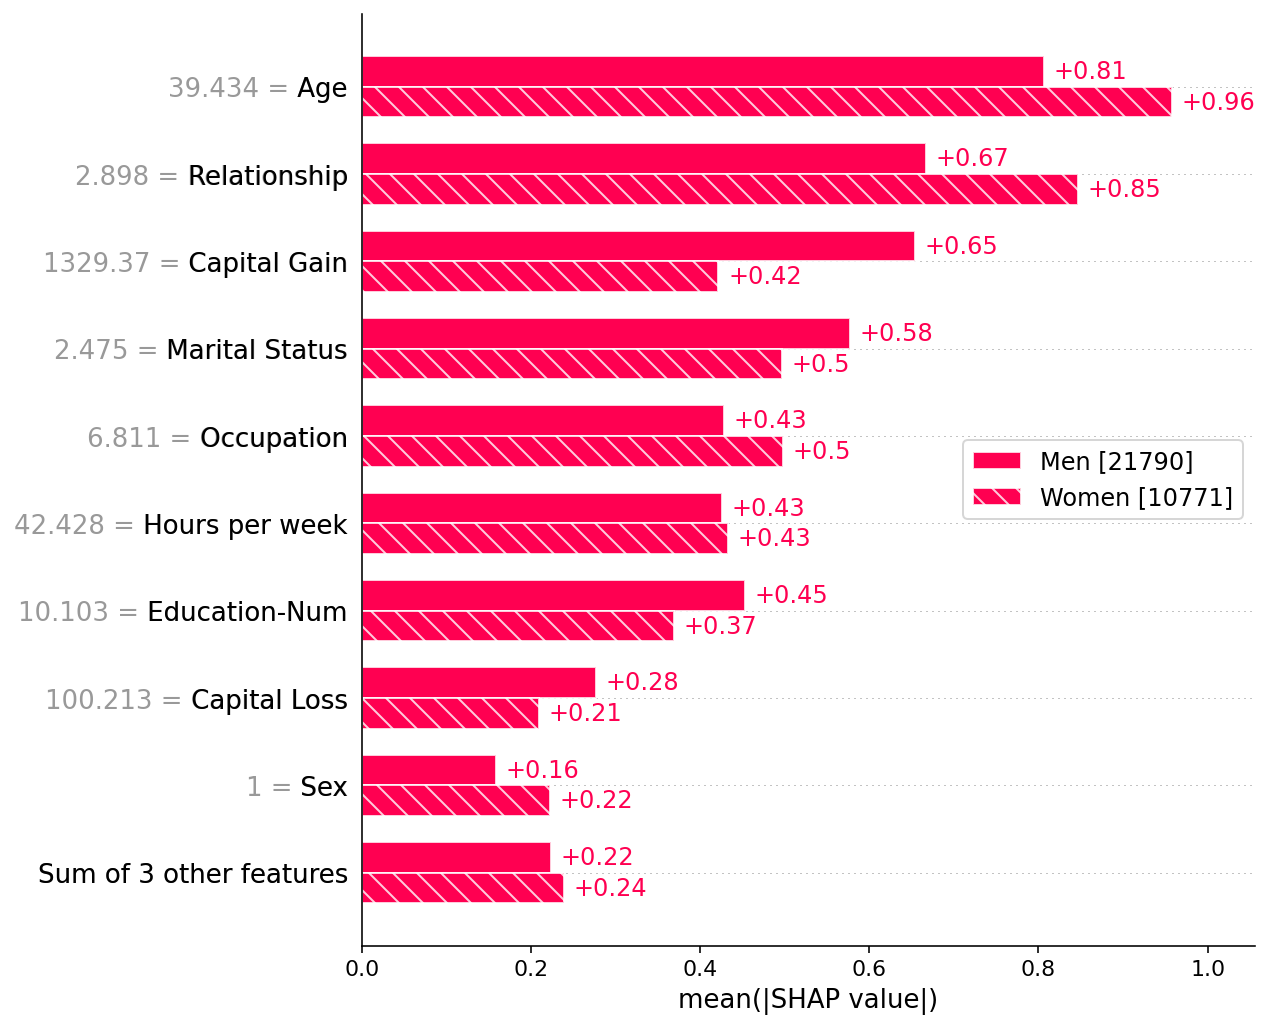
\includegraphics[width=0.43\textwidth]{figs/shap/plots/bar/example_notebooks_api_examples_plots_bar_9_0.png}
        \caption{Global cohort bar plot}
        \label{fig:Cohort-bar}
    \end{figure}
\end{frame}

\begin{frame}{Local feature clustering - Plots}
Often features in datasets are partially or fully redundant with each other. Redundant means that a model could use either feature and still get the same accuracy. To find these features practitioners will often compute correlation matrices among the features, or use some type of clustering method. 
    \begin{figure}[htbp]
        \centering
        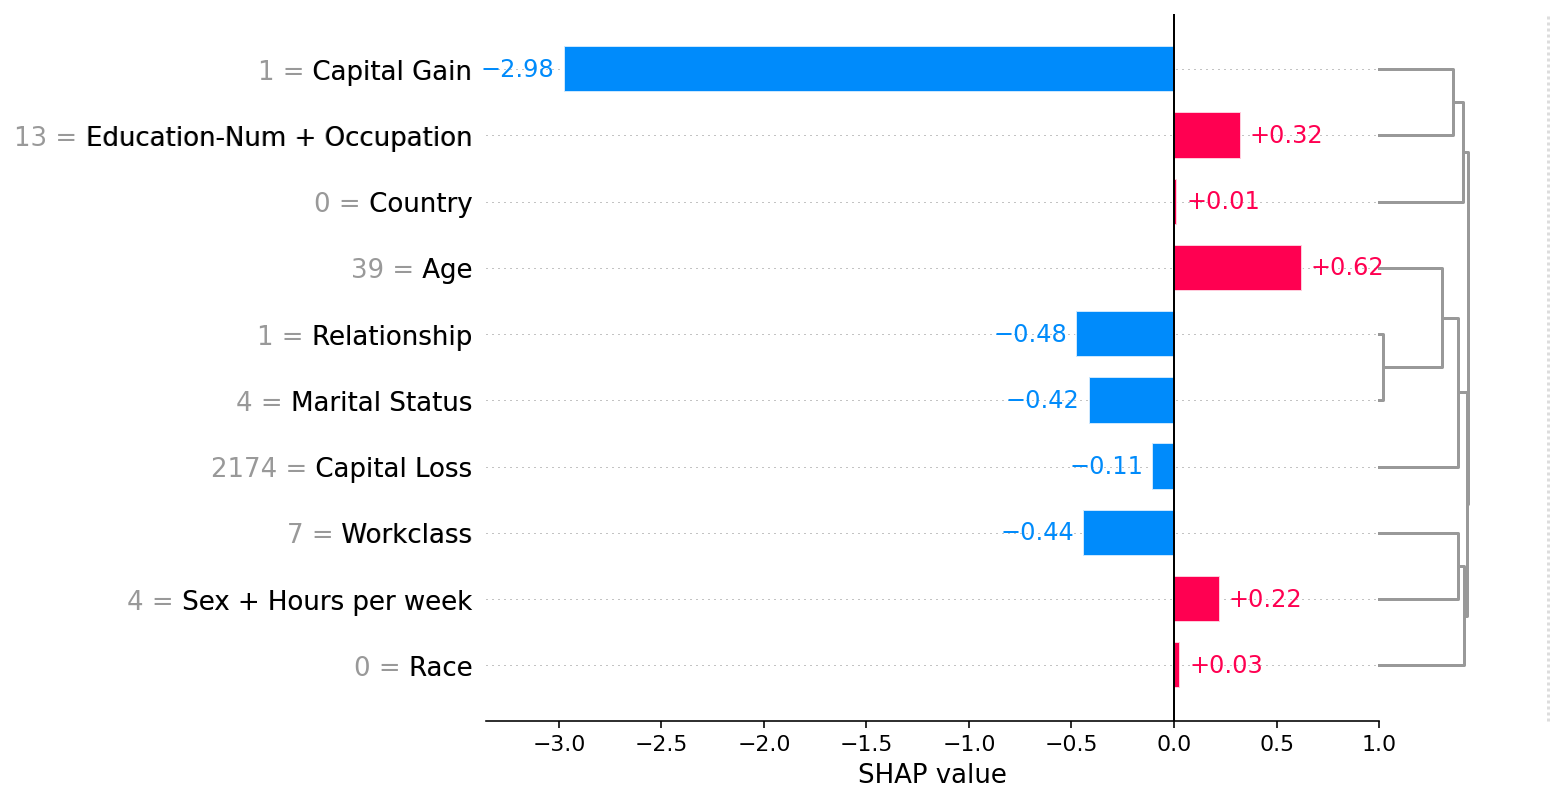
\includegraphics[width=0.6\textwidth]{figs/shap/plots/bar/example_notebooks_api_examples_plots_bar_20_0.png}
        \caption{Local feature clustering}
        \label{fig:local-feature-bar}
    \end{figure}
\end{frame}

\begin{frame}{A simple beeswarm summary plot - Plots}
The beeswarm plot is designed to display an information-dense summary of how the top features in a dataset impact the model’s output. In each instance, the given explanation is represented by a single dot on each feature fow. The x position of the dot is determined by the \ac{SHAP} value of that feature, and dots “pile up” along each feature row to show density. Color is used to display the original value of a feature. In the plot below we can see that Age is the most important feature on average, and then young (blue) people are less likely to make over \$50k.
    \begin{figure}[htbp]
        \centering
        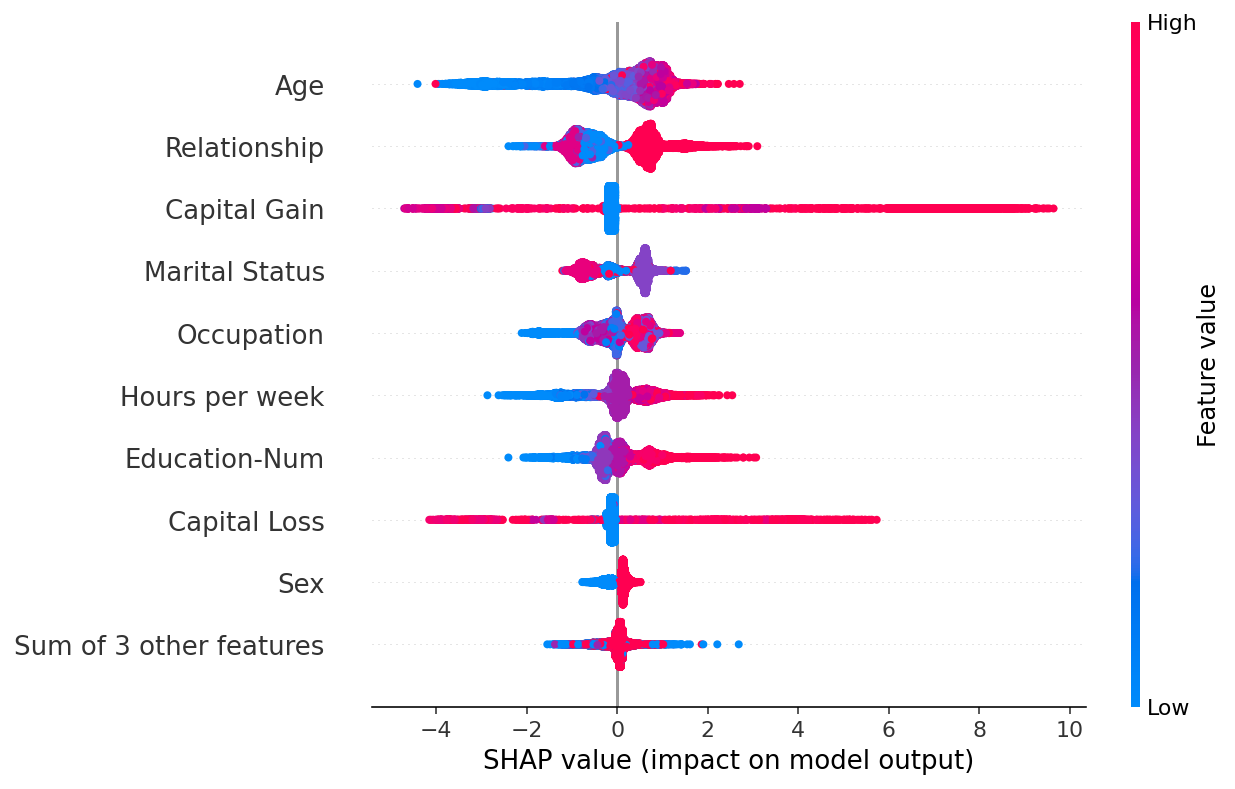
\includegraphics[width=0.38\textwidth]{figs/shap/plots/beeswarm/example_notebooks_api_examples_plots_beeswarm_3_0.png}
        \caption{A simple beeswarm summary plot}
        \label{fig:simple-beeswarm}
    \end{figure}
\end{frame}

\begin{frame}{Feature ordering beeswarm - Plots}
By default the features are ordered using shap\_values.abs.mean(0), which is the mean absolute value of the \ac{SHAP} values for each feature. This order however places more emphasis on broad average impact, and less on rare but high-magnitude impacts. If we want to find features with high impacts for individual people we can instead sort by the max absolute value:
    \begin{figure}[htbp]
        \centering
        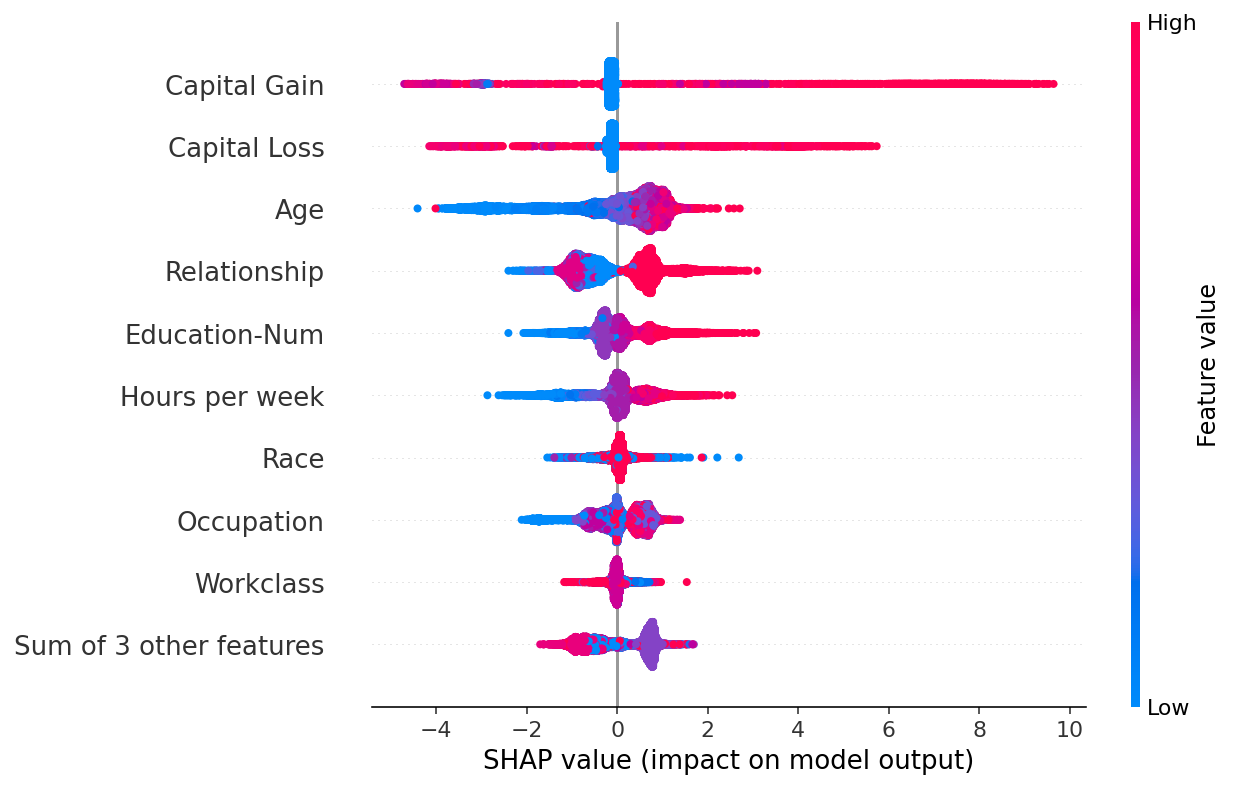
\includegraphics[width=0.50\textwidth]{figs/shap/plots/beeswarm/example_notebooks_api_examples_plots_beeswarm_7_0.png}
        \caption{Feature ordering plot}
        \label{fig:feature-beeswarm}
    \end{figure}
\end{frame}

\begin{frame}{Useful transforms beeswarm - Plots}
Sometimes it is helpful to transform the \ac{SHAP} values before we plot them. Below we plot the absolute value and fix the color to be red. This creates a richer parallel to the standard shap\_values.abs.mean(0) bar plot, since the bar plot just plots the mean value of the dots in the beeswarm plot.
    \begin{figure}[htbp]
        \centering
        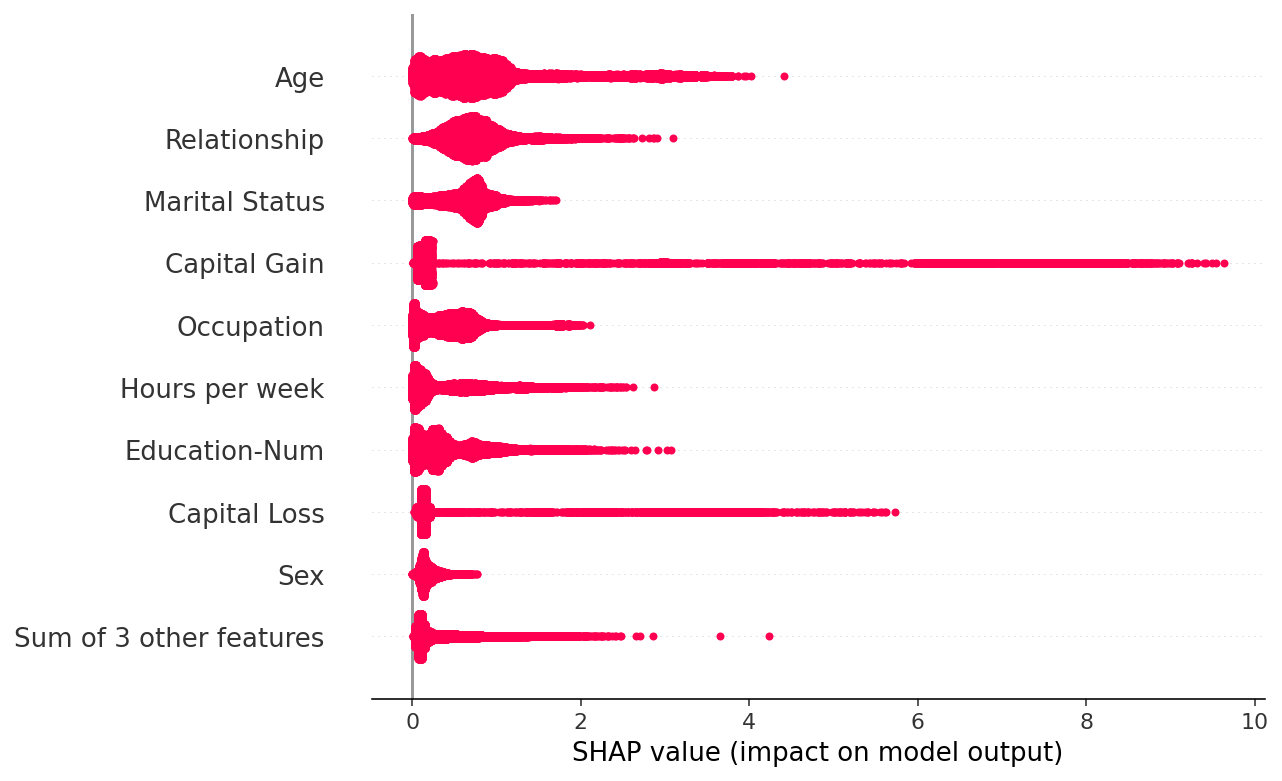
\includegraphics[width=0.52\textwidth]{figs/shap/plots/beeswarm/example_notebooks_api_examples_plots_beeswarm_9_0.png}
        \caption{Useful transforms plot}
        \label{fig:transforms-beeswarm}
    \end{figure}
\end{frame}

\begin{frame}{Custom colors beeswarm - Plots}
By default, beeswarm uses the shap.plots.colors.red\_blue color map, but you can pass any matplotlib color or colormap using the color parameter:
    \begin{figure}[htbp]
        \centering
        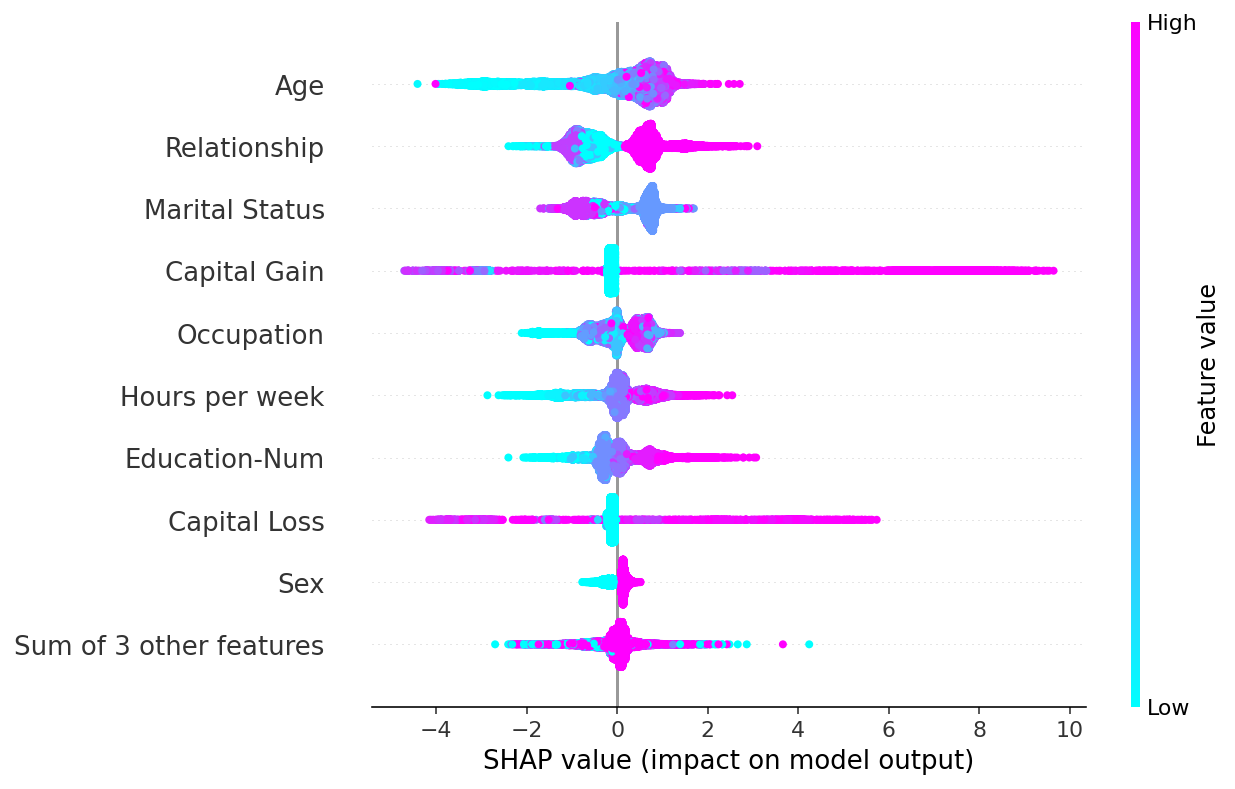
\includegraphics[width=0.6\textwidth]{figs/shap/plots/beeswarm/example_notebooks_api_examples_plots_beeswarm_12_0.png}
        \caption{Custom colors plot}
        \label{fig:custom-beeswarm}
    \end{figure}
\end{frame}

\begin{frame}{Basic decision plot features - Plots}
    Refer to the decision plot of the 20 test observations below. Note: This plot isn’t informative by itself; we use it only to illustrate the primary concepts.
    \begin{itemize}
        \item The x-axis represents the model’s output. In this case, the units are log odds.
        \item The plot is centered on the x-axis at explainer.expected\_value. All \ac{SHAP} values are relative to the model’s expected value like a linear model’s effects are relative to the intercept.
        \item The y-axis lists the model’s features. By default, the features are ordered by descending importance. The importance is calculated over the observations plotted. This is usually different than the importance ordering for the entire dataset. In addition to feature importance ordering, the decision plot also supports hierarchical cluster feature ordering and user-defined feature ordering.
    \end{itemize}
\end{frame}

\begin{frame}{Basic decision plot features - Plots}
    \begin{itemize}
        \item Each observation’s prediction is represented by a colored line. At the top of the plot, each line strikes the x-axis at its corresponding observation’s predicted value. This value determines the color of the line on a spectrum.
        \item Moving from the bottom of the plot to the top, \ac{SHAP} values for each feature are added to the model’s base value. This shows how each feature contributes to the overall prediction. 
        \item At the bottom of the plot, the observations converge at explainer.expected\_value.
    \end{itemize}
\end{frame}

\begin{frame}{Basic decision plot features - Plots}
    \begin{figure}[htbp]
        \centering
        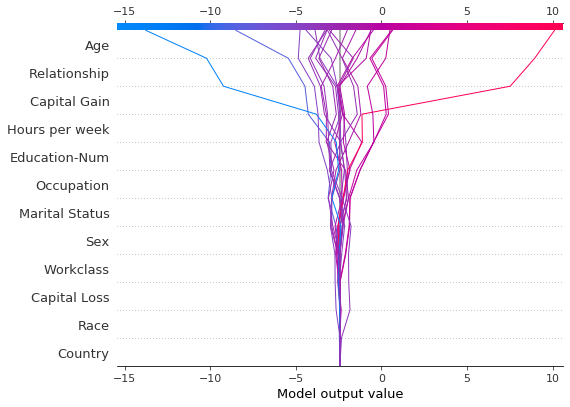
\includegraphics[width=0.67\textwidth]{figs/shap/plots/decision/example_notebooks_api_examples_plots_decision_plot_8_0.png}
        \caption{Basic decision plot features}
        \label{fig:basic-decision}
    \end{figure}
\end{frame}

\begin{frame}{Basic decision plot features - Plots}
Like the force plot, the decision plot supports link='logit' to transform log odds to probabilities.
    \begin{figure}[htbp]
        \centering
        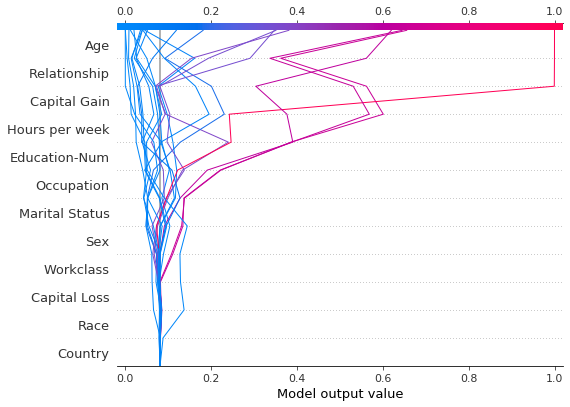
\includegraphics[width=0.59\textwidth]{figs/shap/plots/decision/example_notebooks_api_examples_plots_decision_plot_10_0.png}
        \caption{Basic decision plot features - logit}
        \label{fig:logit-decision}
    \end{figure}
\end{frame}

\begin{frame}{Basic decision plot features - Plots}
Observations can be highlighted using a dotted line style. Here, we highlight a misclassified observation.
    \begin{figure}[htbp]
        \centering
        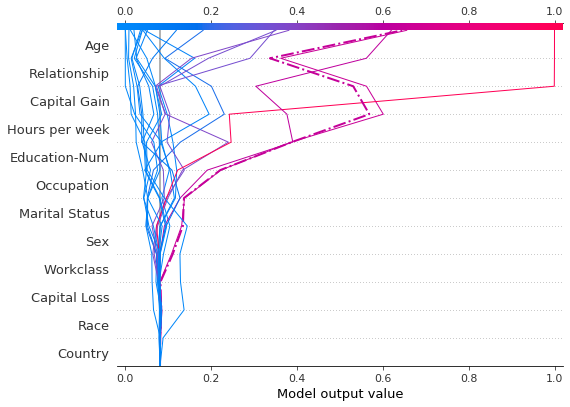
\includegraphics[width=0.55\textwidth]{figs/shap/plots/decision/example_notebooks_api_examples_plots_decision_plot_12_0.png}
        \caption{Basic decision plot features - misclassified observation}
        \label{fig:misclassified-decision}
    \end{figure}
\end{frame}

\begin{frame}{Basic decision plot features - Plots}
Let’s inspect the misclassified observation by plotting it alone. When a single observation is plotted, its corresponding feature values are displayed. Notice that the shape of the line has changed. Why? The feature order has changed on the y-axis based on the feature importance for this lone observation. 
    \begin{figure}[htbp]
        \centering
        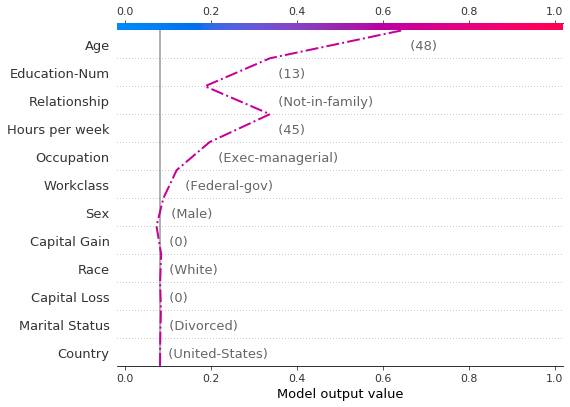
\includegraphics[width=0.45\textwidth]{figs/shap/plots/decision/example_notebooks_api_examples_plots_decision_plot_14_0.png}
        \caption{Basic decision plot features - inspection misclassified observation}
        \label{fig:inspection-misclassified-decision}
    \end{figure}
\end{frame}

\begin{frame}{Basic decision plot features - Plots}
A force plot for the misclassified observation is shown below. In this case, the decision plot and the force plot are both effective at showing how the model arrived at its decision.
    \begin{figure}[htbp]
        \centering
        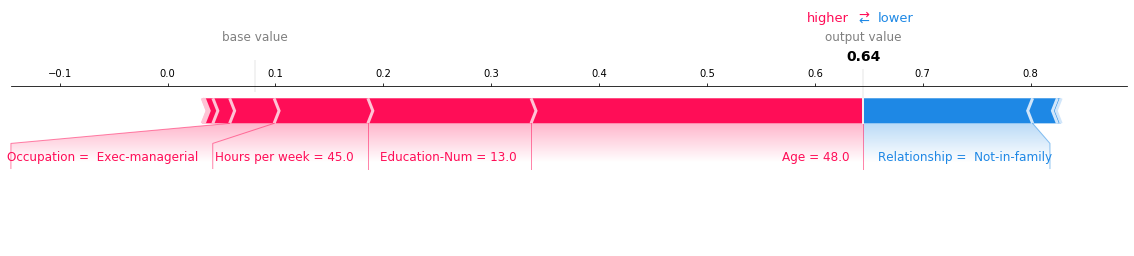
\includegraphics[width=0.9\textwidth]{figs/shap/plots/decision/example_notebooks_api_examples_plots_decision_plot_16_0.png}
        \caption{Basic decision plot features - force plot}
        \label{fig:force-inspection-misclassified-decision}
    \end{figure}
\end{frame}

\begin{frame}{HeatMap - Plots}
Passing a matrix of \ac{SHAP} values to the heatmap plot function creates a plot with the instances on the x-axis, the model inputs on the y-axis, and the \ac{SHAP} values encoded on a color scale. By default, the samples are ordered using shap.order.hclust, which orders the samples based on a hierarchical clustering by their explanation similarity. This results in samples that have the same model output for the same reason getting grouped (such as people with a high impact from capital gain in the plot below).

The output of the model is shown above the heatmap matrix (centered around the explanation’s .base\_value), and the global importance of each model input is shown as a bar plot on the right-hand side of the plot (by default this is the shap.order.abs.mean measure of overall importance).
\end{frame}

\begin{frame}{HeatMap - Plots}
    \begin{figure}[htbp]
        \centering
        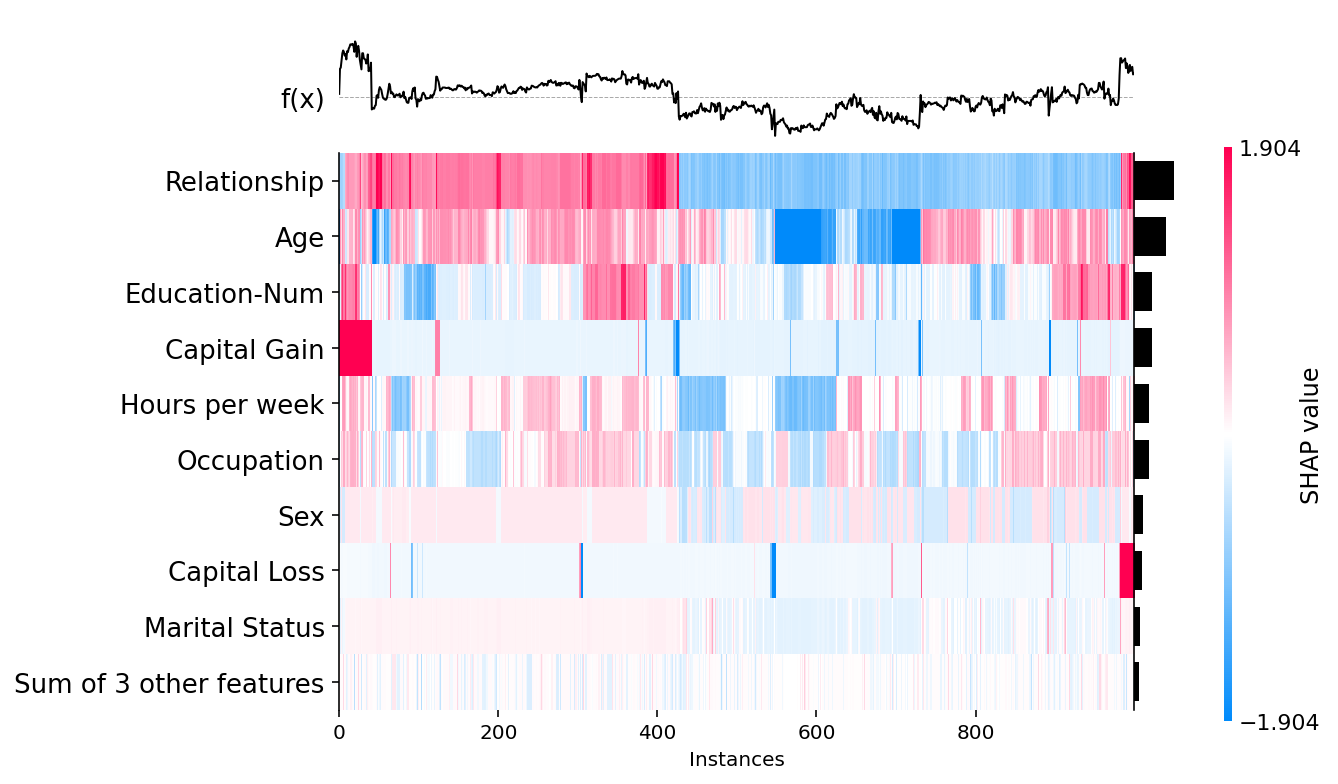
\includegraphics[width=0.8\textwidth]{figs/shap/plots/heatmap/example_notebooks_api_examples_plots_heatmap_3_0.png}
        \caption{HeatMap plot}
        \label{fig:heatmap}
    \end{figure}
\end{frame}

\begin{frame}{HeatMap - Plots}
    \begin{figure}[htbp]
        \centering
        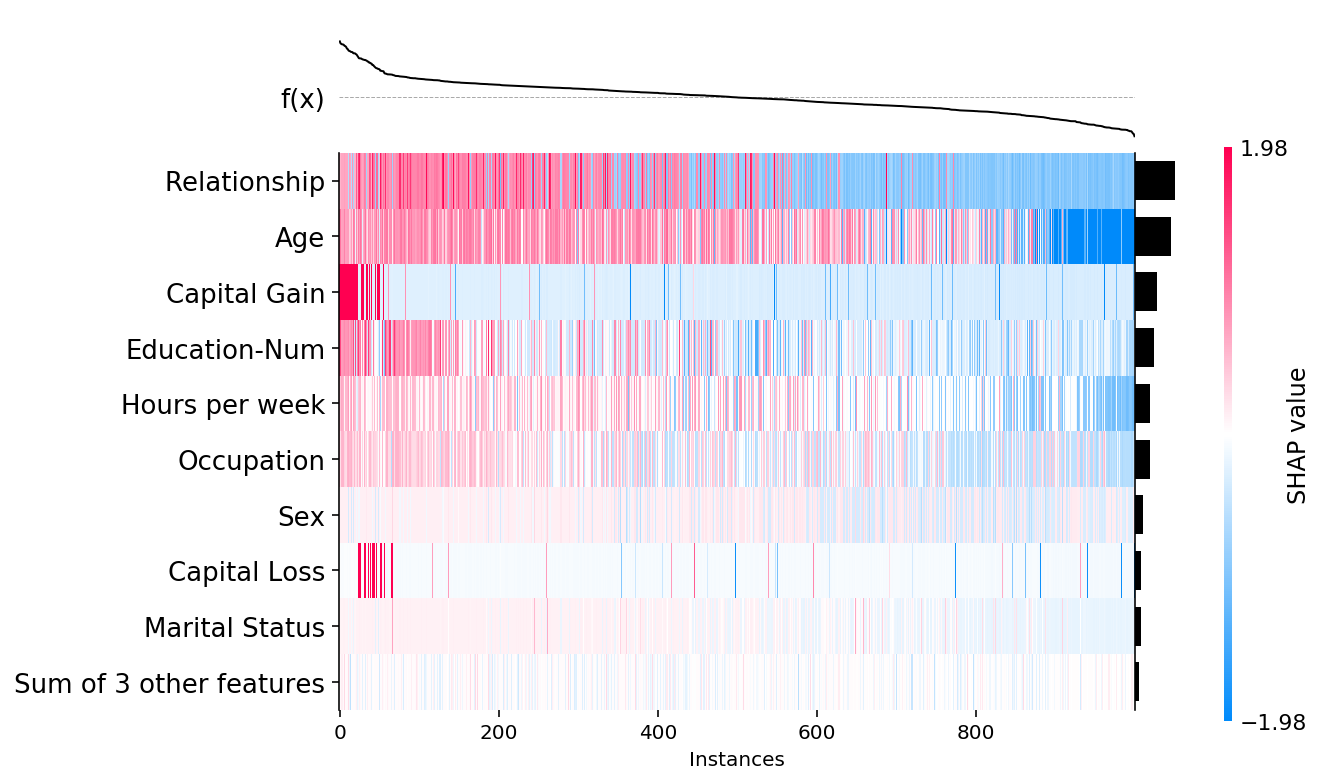
\includegraphics[width=0.8\textwidth]{figs/shap/plots/heatmap/example_notebooks_api_examples_plots_heatmap_9_0.png}
        \caption{Changing sort order and global feature importance values - HeatMap plot}
        \label{fig:sort-heatmap}
    \end{figure}
\end{frame}

\begin{frame}{Image - Plots}
Highlights important regions in the images that contribute to the predictions of the ResNet50 model.
    \begin{figure}[htbp]
        \centering
        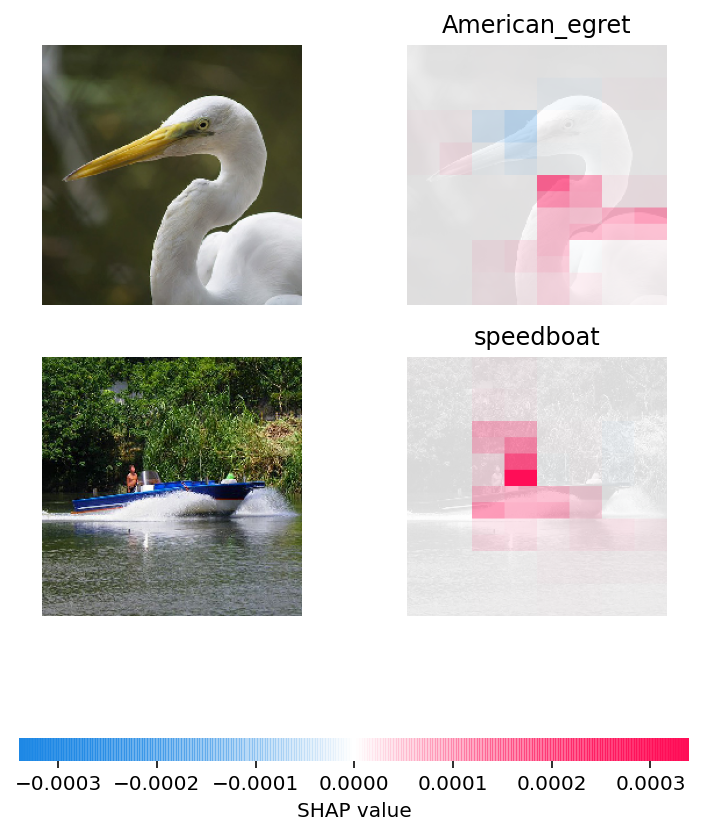
\includegraphics[width=0.32\textwidth]{figs/shap/plots/image/example_notebooks_api_examples_plots_image_1_3.png}
        \caption{The activations in image}
        \label{fig:activations-image}
    \end{figure}
\end{frame}

\begin{frame}{Simple dependence scatter plot - Plots}
A dependence scatter plot shows the effect a single feature has on the predictions made by the model. In this example, the log-odds of making over 50k increases significantly between age 20 and 40.

    \begin{itemize}
        \item Each dot is a single prediction (row) from the dataset.
        \item The x-axis is the value of the feature (from the X matrix, stored in shap\_values.data).
        \item The y-axis is the \ac{SHAP} value for that feature (stored in shap\_values.values), which represents how much knowing that feature’s value changes the output of the model for that sample’s prediction. For this model, the units are log-odds of making over 50k annually.
        \item The light grey area at the bottom of the plot is a histogram showing the distribution of data values.
    \end{itemize}
\end{frame}

\begin{frame}{Simple dependence scatter plot - Plots}
    \begin{figure}[htbp]
        \centering
        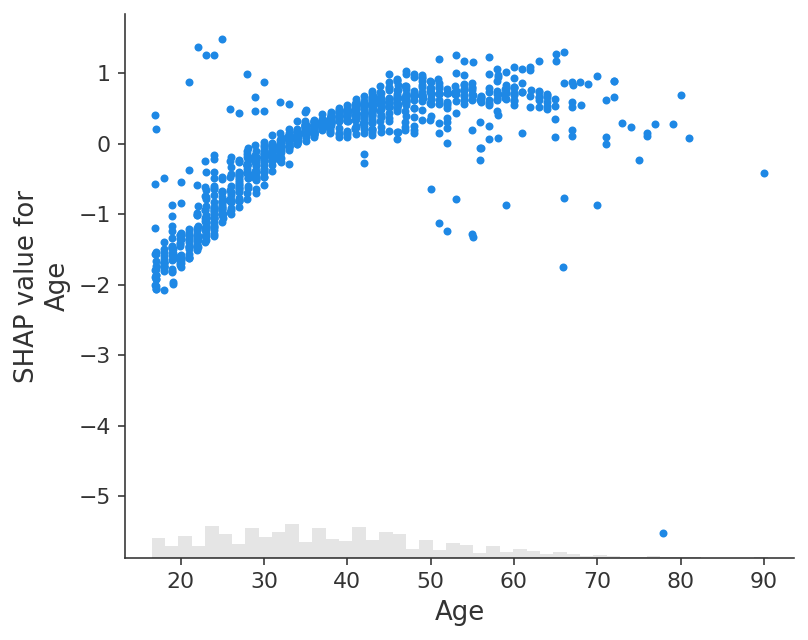
\includegraphics[width=0.6\textwidth]{figs/shap/plots/scatter/example_notebooks_api_examples_plots_scatter_3_0.png}
        \caption{\ac{SHAP} values explanation corresponding to the "Age" feature}
        \label{fig:scatter}
    \end{figure}
\end{frame}

\begin{frame}{Using color to highlight interaction effects in scatter - Plots}

The vertical dispersion in the plot above shows that the same value for the Age feature can have a different impact on the model’s output for different people. This means there are non-linear interaction effects in the model between Age and other features (otherwise the scatter plot would perfectly follow the line given by shap.plots.partial\_dependence).

To show which feature may be driving these interaction effects we can color our Age dependence scatter plot by another feature. If we pass the entire Explanation object to the color parameter then the scatter plot attempts to pick out the feature column with the strongest interaction with Age. If an interaction effect is present between this other feature and the feature we are plotting it will show up as a distinct vertical pattern of coloring. For the example below, 20-year-olds with a high level of education are less likely to make over \$50k than 20-year-olds with a low level of education. This suggests an interaction effect between Education-Num and Age.
\end{frame}

\begin{frame}{Using color to highlight interaction effects in scatter - Plots}
    \begin{figure}[htbp]
        \centering
        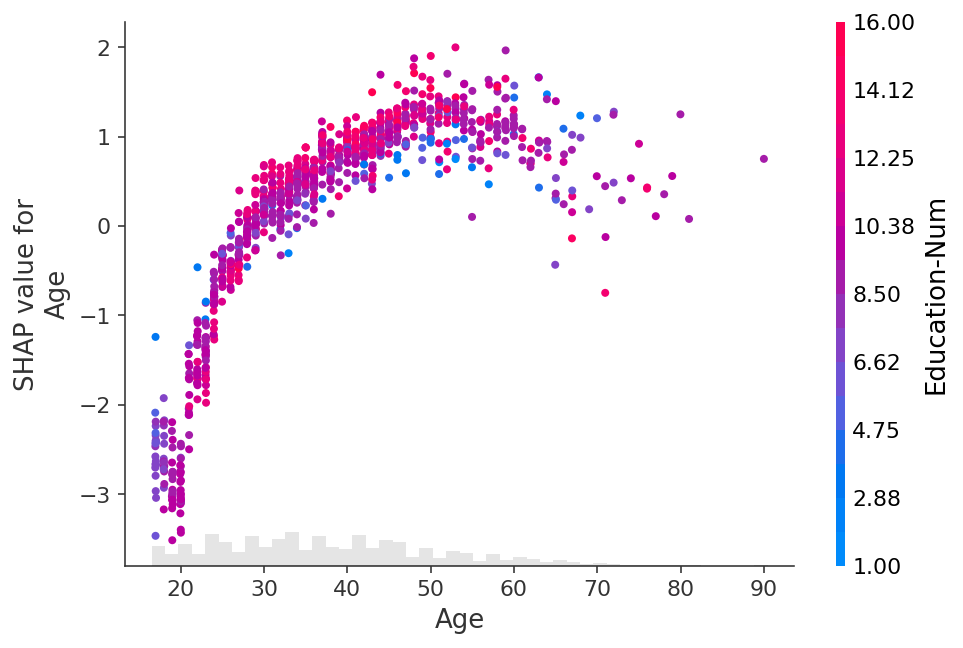
\includegraphics[width=0.7\textwidth]{figs/shap/plots/scatter/example_notebooks_api_examples_plots_scatter_5_0.png}
        \caption{Interaction effect between Education-Num and Age}
        \label{fig:interaction-scatter}
    \end{figure}
\end{frame}

\begin{frame}{Using color to highlight interaction effects in scatter - Plots}

To explicitly control which feature is used for coloring you can pass a specific feature column to the color parameter.

    \begin{figure}[htbp]
        \centering
        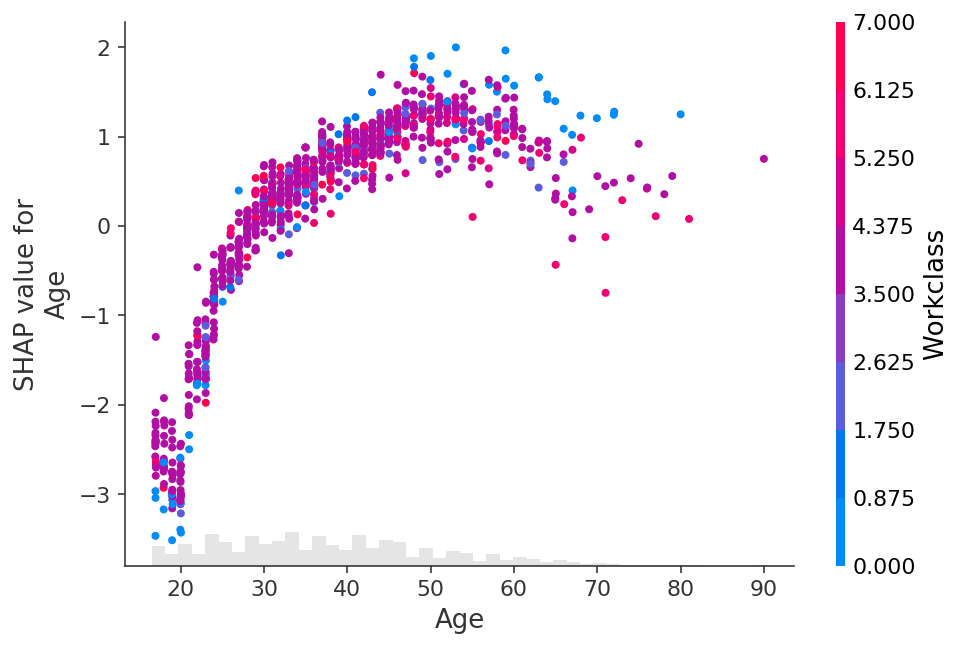
\includegraphics[width=0.55\textwidth]{figs/shap/plots/scatter/example_notebooks_api_examples_plots_scatter_7_0.png}
        \caption{Interaction effect between Education-Num, Age, and Workclass}
        \label{fig:color-interaction-scatter}
    \end{figure}
\end{frame}

\begin{frame}{Using color to highlight interaction effects in scatter - Plots}

We see that the Workclass feature is encoded with a number for the sake of the XGBoost model. When plotting though we often would rather use the original string values before they were categorically encoded. To do this we can set the .display\_data property of the Explanation object to a parallel version of the data we would like displayed in plots.

    \begin{figure}[htbp]
        \centering
        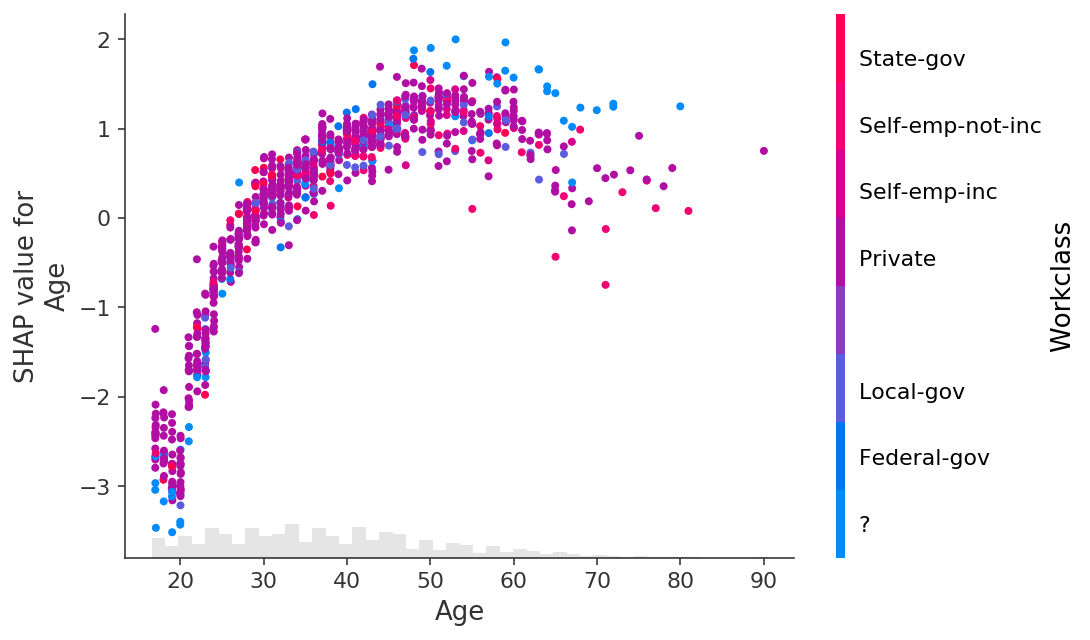
\includegraphics[width=0.52\textwidth]{figs/shap/plots/scatter/example_notebooks_api_examples_plots_scatter_9_0.png}
        \caption{Interaction effect between Education-Num, Age, and Workclass with property}
        \label{fig:property-color-interaction-scatter}
    \end{figure}
\end{frame}

\begin{frame}{Single instance text plot - Plots}

When we pass a single instance to the text plot we get the importance of each token overlayed on the original text that corresponds to that token. Red regions correspond to parts of the text that increase the output of the model when they are included, while blue regions decrease the output of the model when they are included. In the context of the sentiment analysis model here red corresponds to a more positive review and blue a more negative review.

The force plot above the text is designed to provide an overview of how all the parts of the text combine to produce the model’s output.
\end{frame}


\begin{frame}{Single instance text plot - Plots}

    \begin{figure}[htbp]
        \centering
        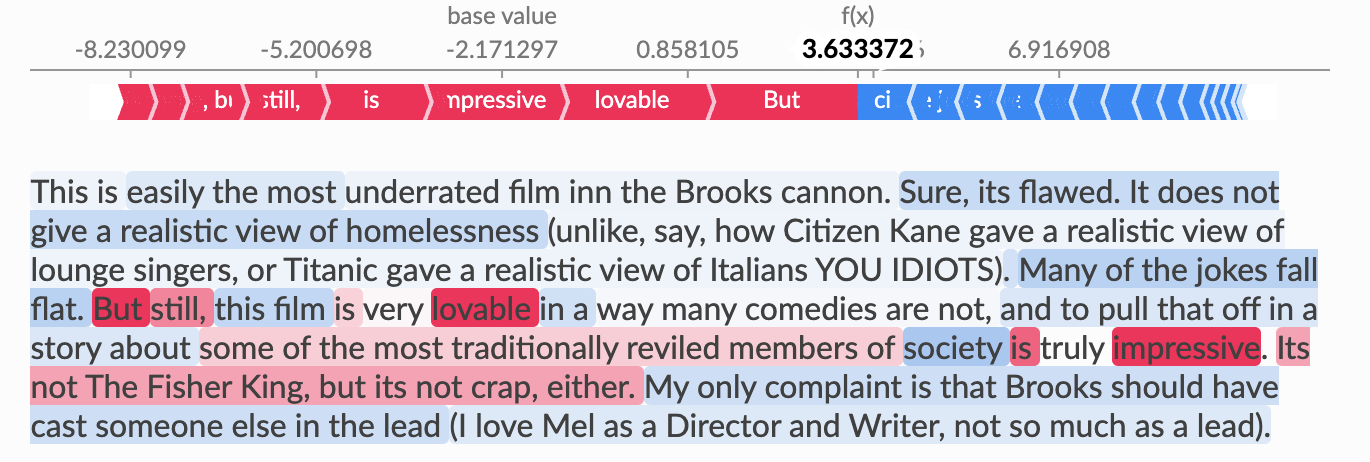
\includegraphics[width=1\textwidth]{figs/shap/plots/text/sample_text.png}
        \caption{Sample text}
        \label{fig:sample-text}
    \end{figure}
\end{frame}

\begin{frame}{Multiple instance text plot - Plots}

When we pass a multi-row explanation object to the text plot we get the single instance plots for each input instance scaled so they have consistent comparable x-axis and color ranges.

    \begin{figure}[htbp]
        \centering
        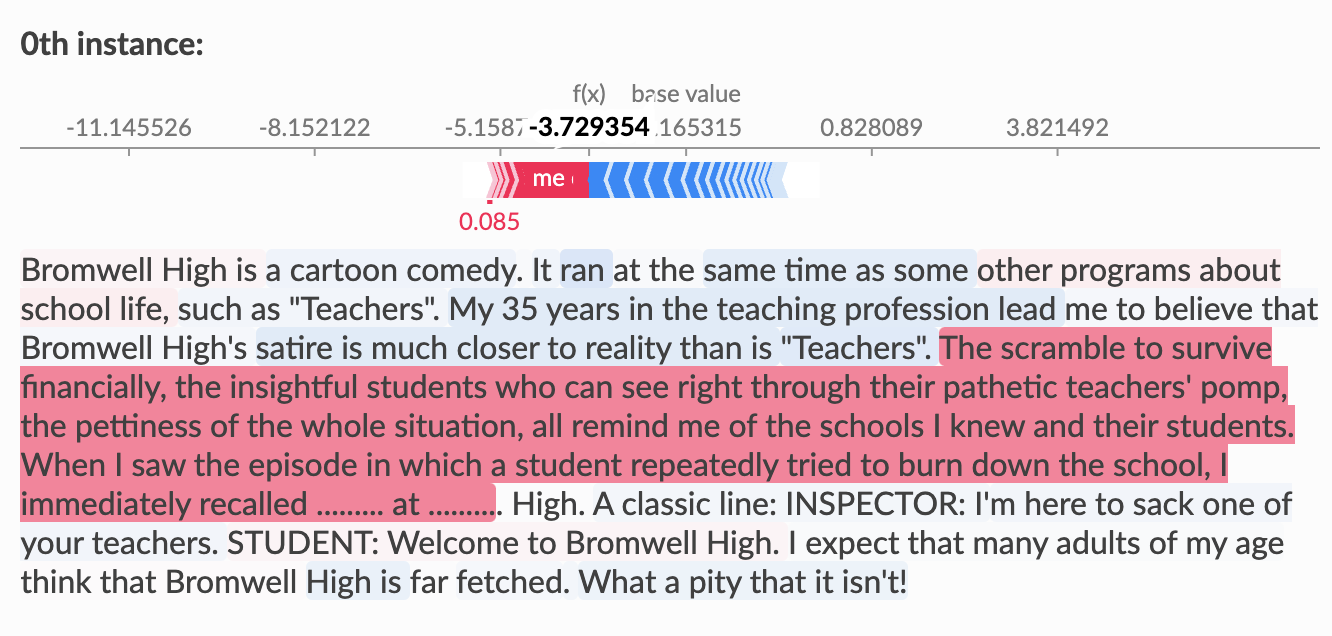
\includegraphics[width=0.8\textwidth]{figs/shap/plots/text/sample_text_0th.png}
        \caption{0th instance}
        \label{fig:0th-sample-text}
    \end{figure}
\end{frame}

\begin{frame}{Multiple instance text plot - Plots}
    \begin{figure}[htbp]
        \centering
        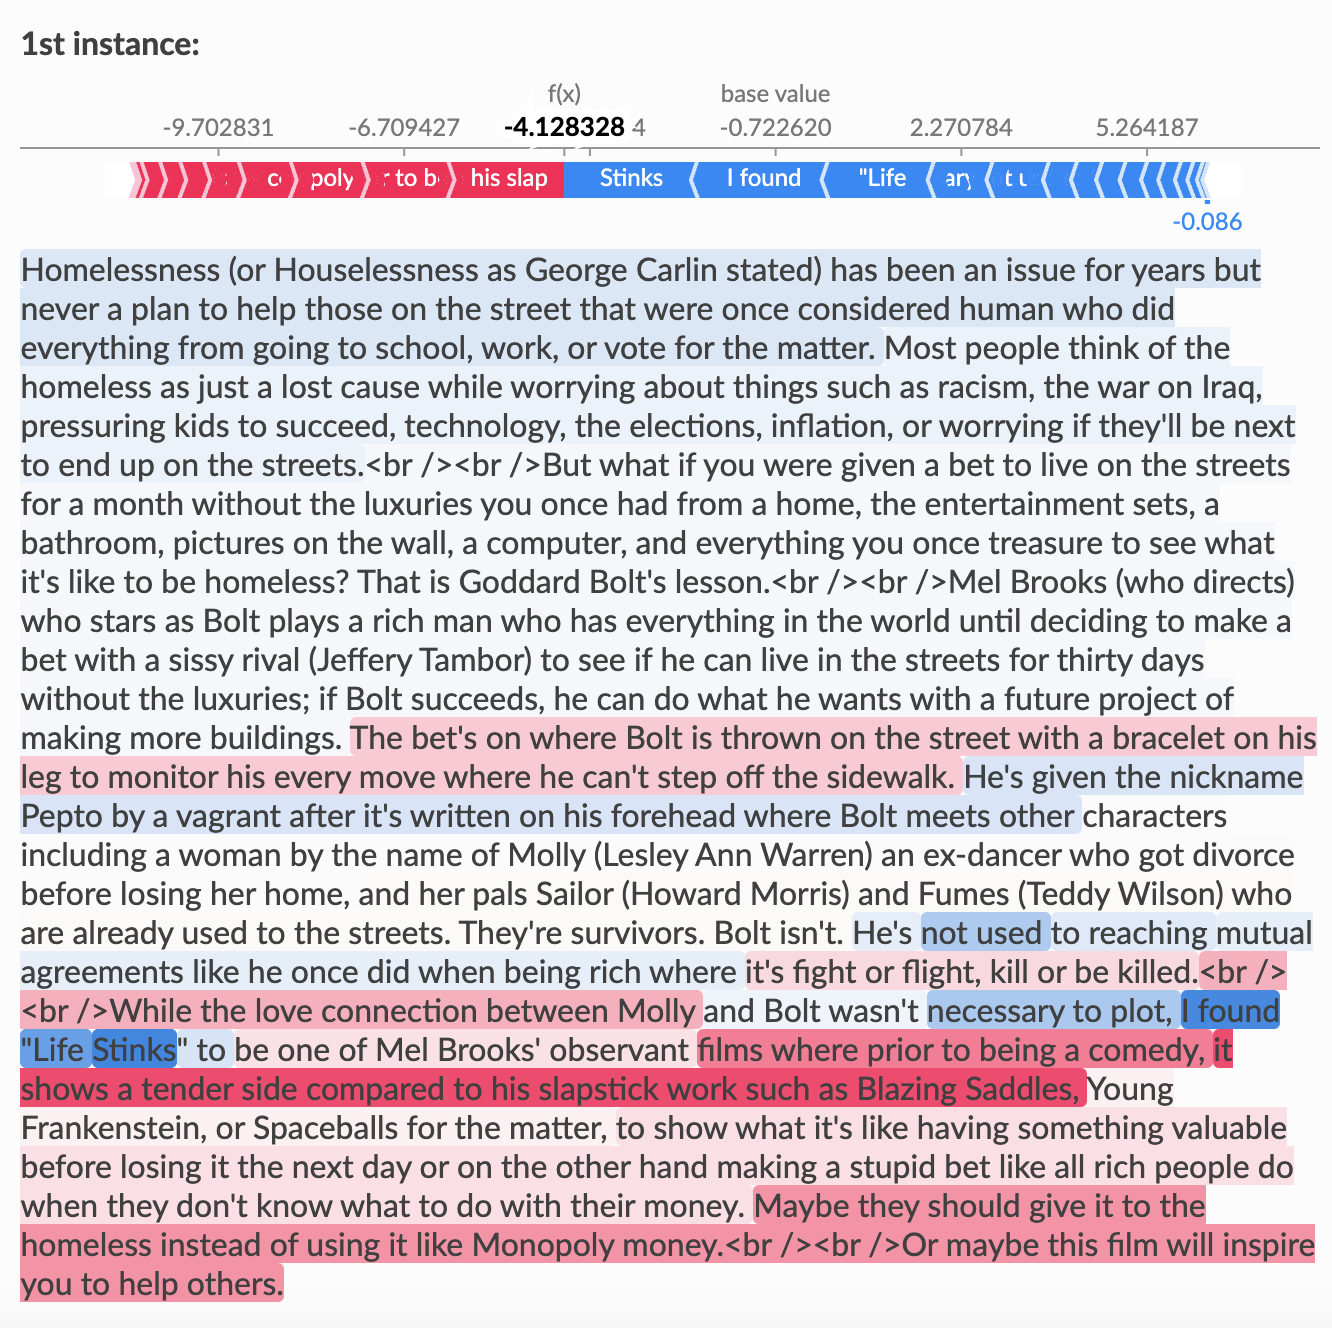
\includegraphics[width=0.48\textwidth]{figs/shap/plots/text/sample_text_1st.png}
        \caption{1st instance}
        \label{fig:1st-sample-text}
    \end{figure}
\end{frame}

\begin{frame}{Multiple instance text plot - Plots}
    \begin{figure}[htbp]
        \centering
        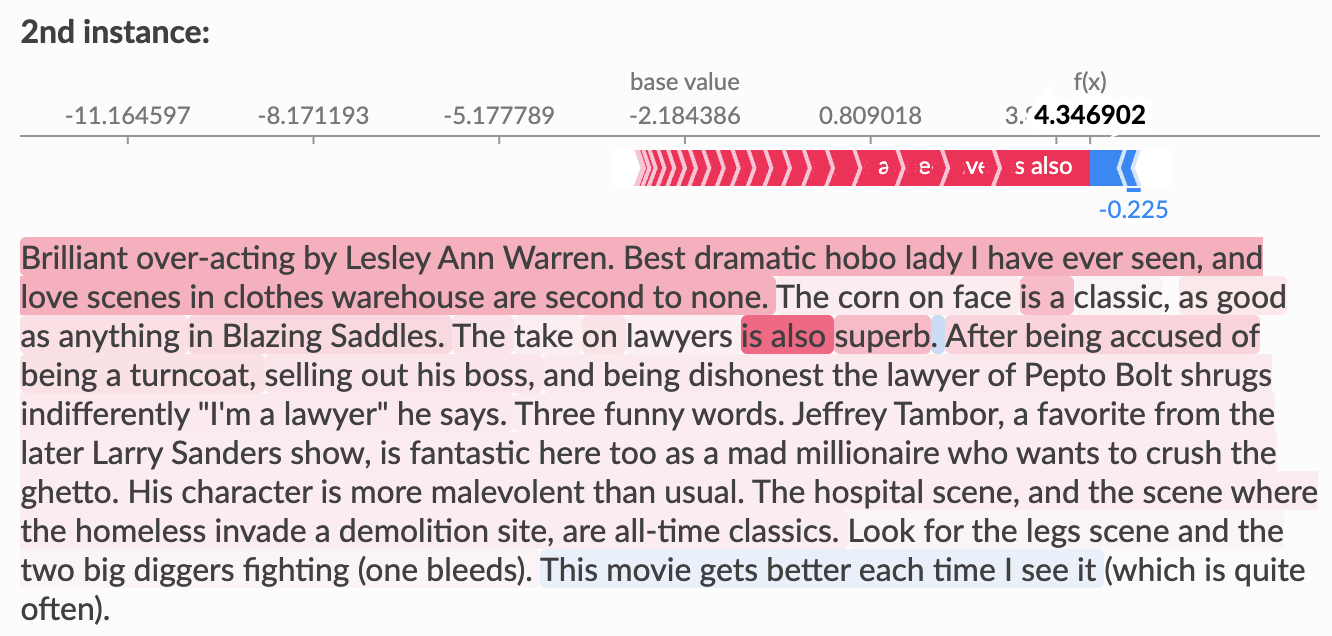
\includegraphics[width=1\textwidth]{figs/shap/plots/text/sample_text_2nd.png}
        \caption{2nd instance}
        \label{fig:2nd-sample-text}
    \end{figure}
\end{frame}

\begin{frame}{Summarizing text explanations - Plots}

While plotting several instance-level explanations using the text plot can be very informative, sometimes you want global summaries of the impact of tokens over a large set of instances. If there are hierarchical values present in the Explanation object then any large groups are divided up and each token in the group is given an equal share of the overall group importance value.

    \begin{figure}[htbp]
        \centering
        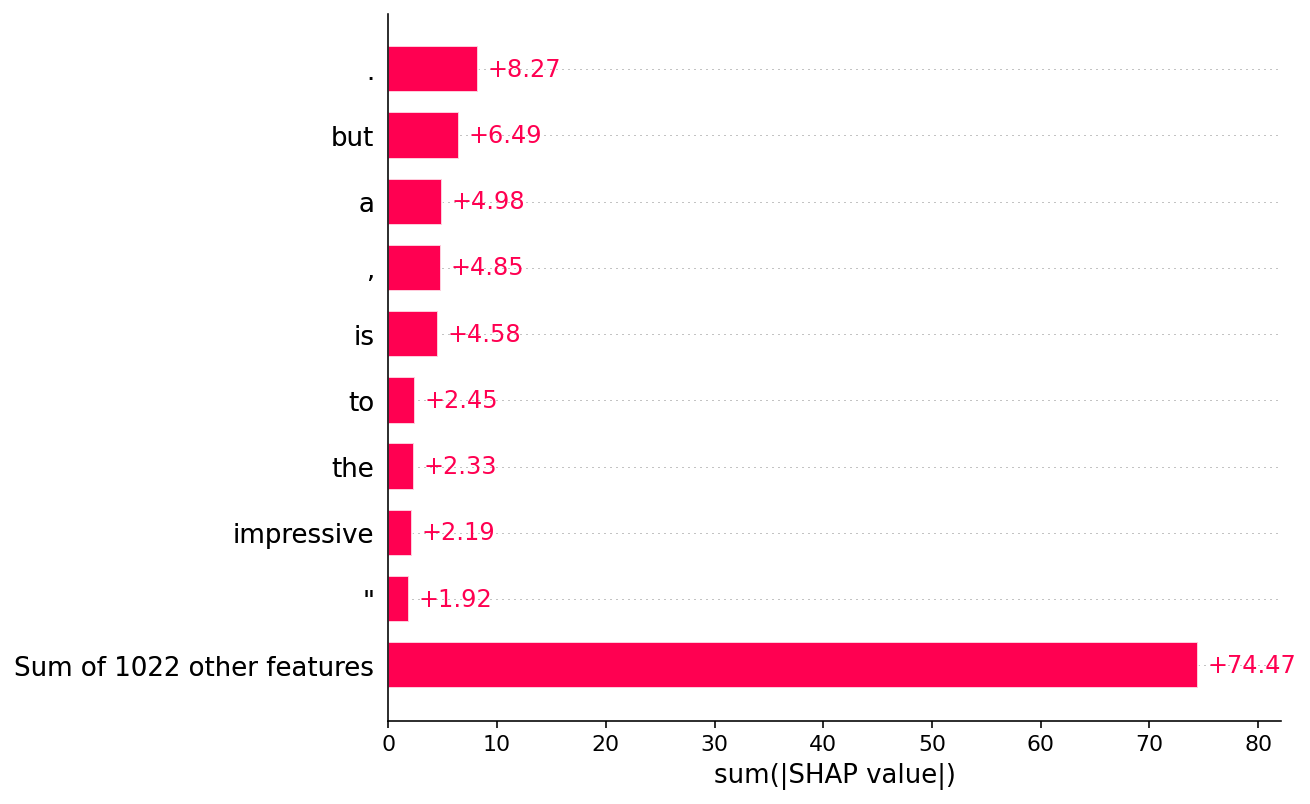
\includegraphics[width=0.45\textwidth]{figs/shap/plots/text/example_notebooks_api_examples_plots_text_7_0.png}
        \caption{Tokens in text}
        \label{fig:tokens-text}
    \end{figure}
\end{frame}

\begin{frame}{Summarizing text explanations - Plots}

You can also slice out a single token from all the instances by using that token as an input name (note that the gray values to the left of the input names are the original text that the token was generated from).

    \begin{figure}[htbp]
        \centering
        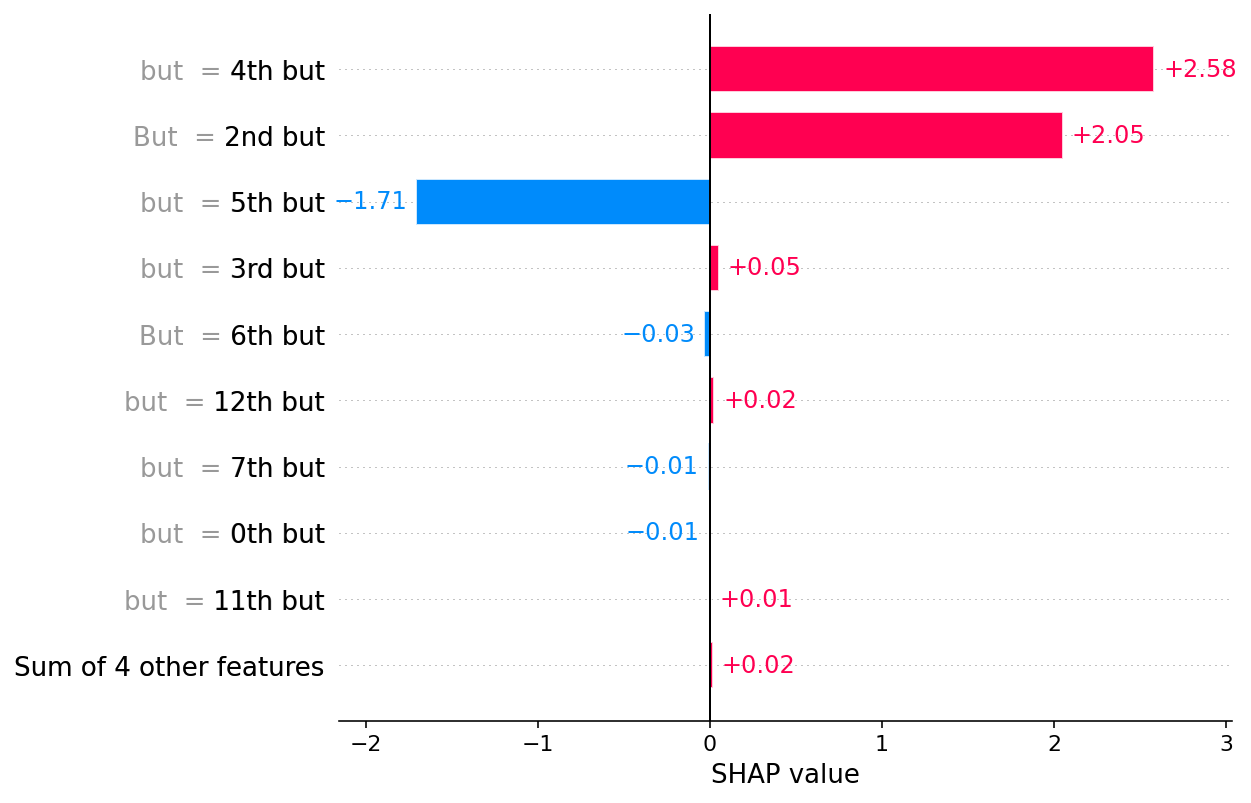
\includegraphics[width=0.55\textwidth]{figs/shap/plots/text/example_notebooks_api_examples_plots_text_11_0.png}
        \caption{Tokens in text from all instances}
        \label{fig:instances-tokens-text}
    \end{figure}
\end{frame}

\begin{frame}{Text-To-Text Visualization - Plots}

Text-to-text visualization contains the input text to the model on the left side and the output text on the right side (in the default layout). On hovering over a token on the right (output) side the importance of each input token is overlayed on it, and is signified by the background color of the token. Red regions correspond to parts of the text that increase the output of the model when they are included, while blue regions decrease the output of the model when they are included.

Note that similar to the single output plots described above, importance values returned for text models are often hierarchical and follow the structure of the text. Small groups of tokens with strong non-linear effects among them will be auto-merged together to form coherent chunks. Similarly, The explainer may not have completely enumerated all possible token perturbations and so has treated chunks of the text as essentially a single unit. This preprocessing is done for each output token, and the merging behavior can differ for each output token since the interaction effects might be different for each output token. The merged chunks can be viewed by hovering over the input text, once an output token is anchored. All the tokens of a merged chunk are made bold.
\end{frame}

\begin{frame}{Text-To-Text Visualization - Plots}
    \begin{figure}[htbp]
        \centering
        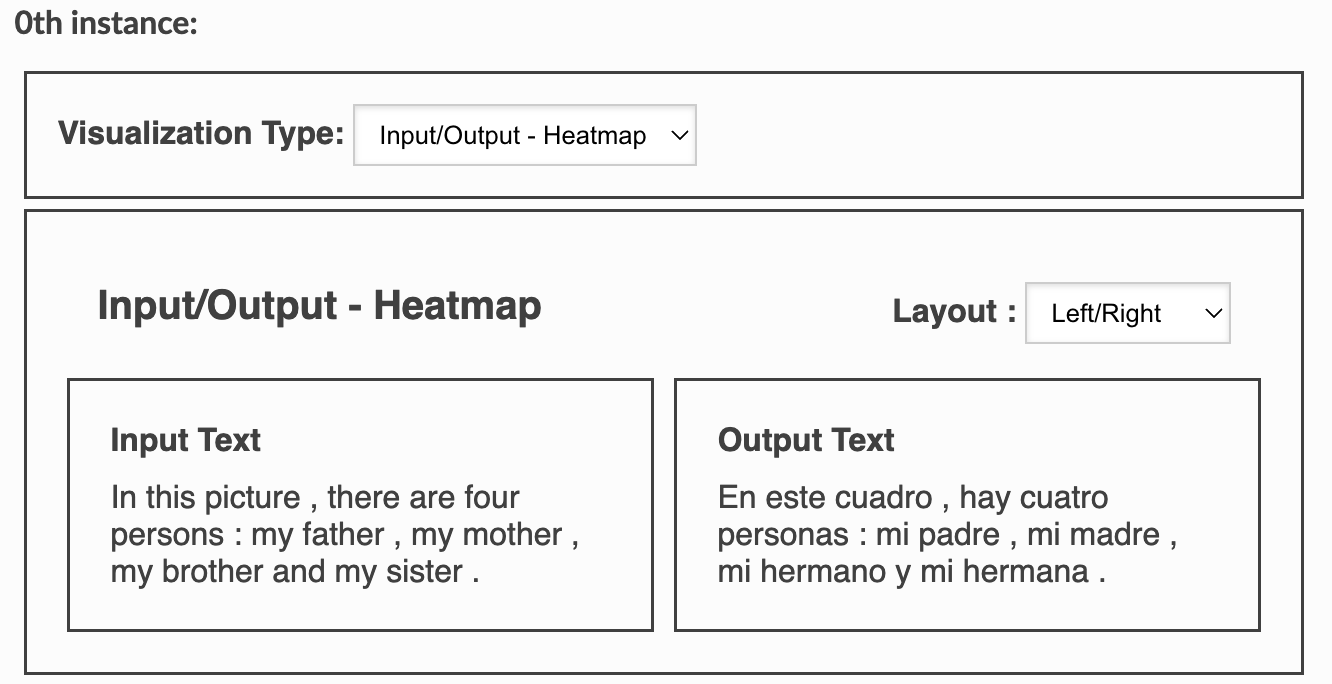
\includegraphics[width=0.9\textwidth]{figs/shap/plots/text/text-to-text.png}
        \caption{Text-To-Text Visualization}
        \label{fig:text-to-text-view}
    \end{figure}
\end{frame}

\begin{frame}{Text-To-Text Visualization - Plots}
    \begin{figure}[htbp]
        \centering
        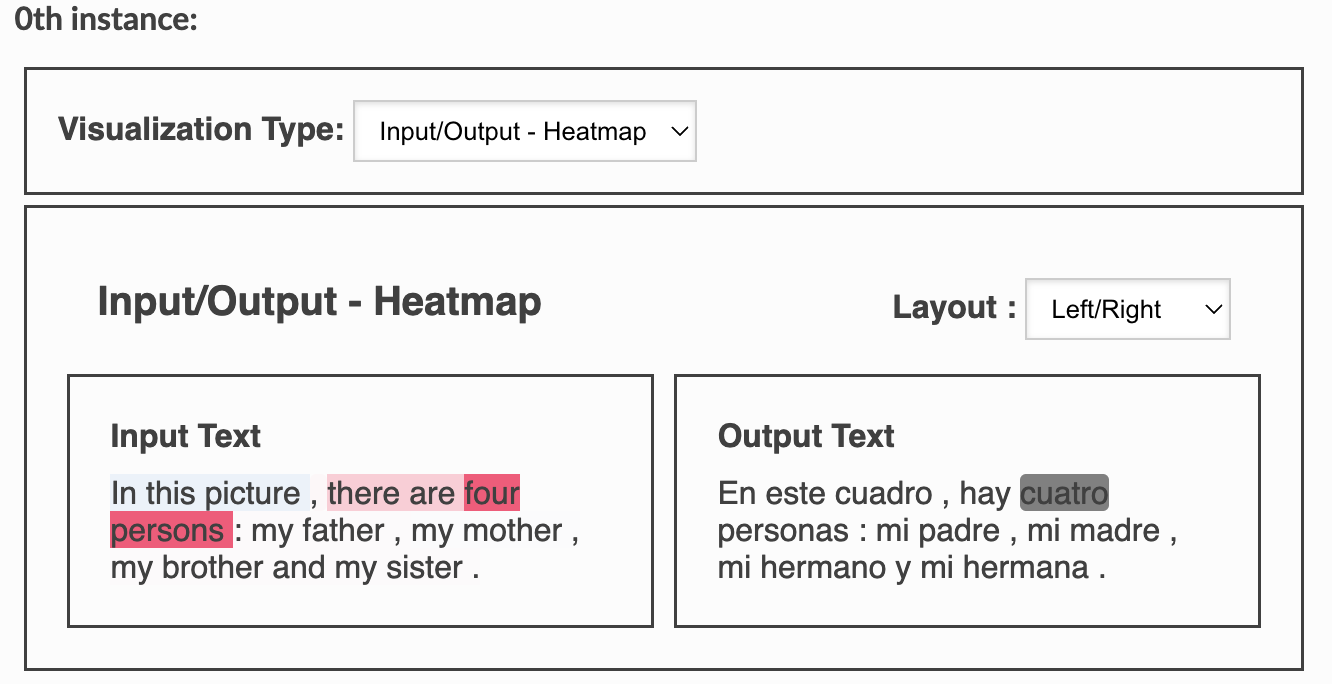
\includegraphics[width=0.9\textwidth]{figs/shap/plots/text/text-to-text-2.png}
        \caption{Text-To-Text Visualization and Interaction}
        \label{fig:text-to-text-view-int}
    \end{figure}
\end{frame}

\begin{frame}{A simple violin summary plot - Plots}
    The violin summary plot offers a compact representation of the distribution and variability of \ac{SHAP} values for each feature. Individual violin plots are stacked by the importance of the particular feature on model output (sum of the absolute values of the \ac{SHAP} values per feature).
    
    Violin plots use “violin-shaped” figures to display the distribution and density of \ac{SHAP} values for their respective feature. The violins can therefore provide insights into the range, variability, skewness, symmetry, and multimodality of the \ac{SHAP} value distribution for a specific feature.
    
    The overall violin summary plot allows for comparisons in feature importance. Wider violins indicate higher density and more frequent values, thus providing insights into the relative importance of each feature in the model output.
\end{frame}

\begin{frame}{A simple violin summary plot - Plots}

    \begin{figure}[htbp]
        \centering
        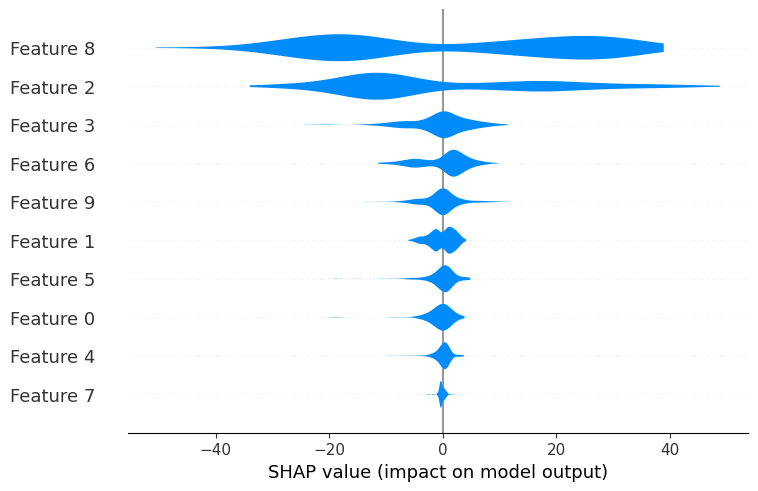
\includegraphics[width=0.7\textwidth]{figs/shap/plots/violin/example_notebooks_api_examples_plots_violin_3_0.png}
        \caption{Simple violin plot}
        \label{fig:simple-violin-plot}
    \end{figure}
\end{frame}

\begin{frame}{A simple violin summary plot - Plots}

    \begin{figure}[htbp]
        \centering
        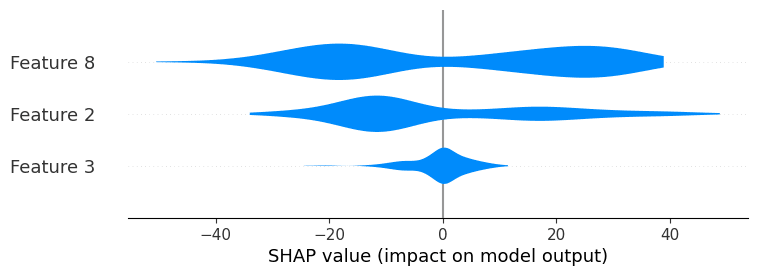
\includegraphics[width=1\textwidth]{figs/shap/plots/violin/example_notebooks_api_examples_plots_violin_5_0.png}
        \caption{Simple violin adjusted size plot}
        \label{fig:simple-violin-plot-adjusted-size}
    \end{figure}
\end{frame}

\begin{frame}{A simple violin summary plot - Plots}

    \begin{figure}[htbp]
        \centering
        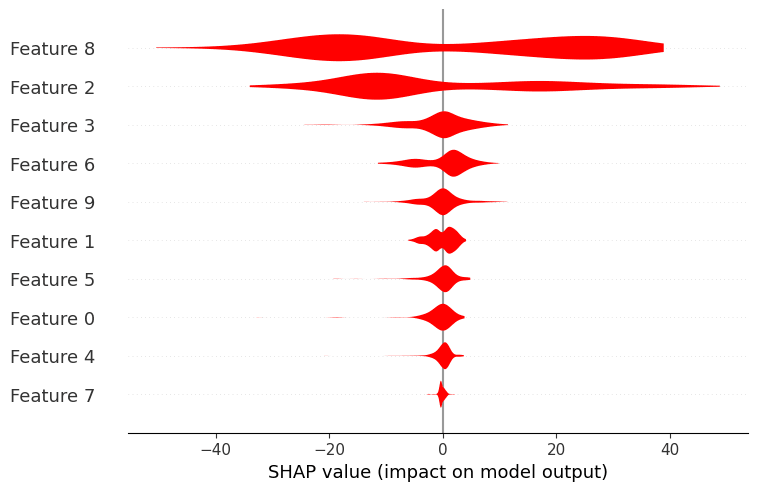
\includegraphics[width=0.7\textwidth]{figs/shap/plots/violin/example_notebooks_api_examples_plots_violin_7_0.png}
        \caption{Simple violin changed color plot}
        \label{fig:simple-violin-plot-color}
    \end{figure}
\end{frame}

\begin{frame}{A simple violin summary plot - Plots}

    \begin{figure}[htbp]
        \centering
        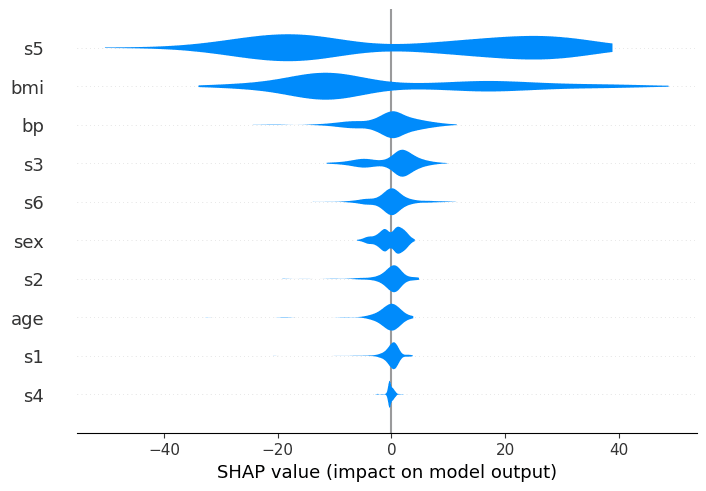
\includegraphics[width=0.65\textwidth]{figs/shap/plots/violin/example_notebooks_api_examples_plots_violin_9_0.png}
        \caption{Simple violin with feature name plot}
        \label{fig:simple-violin-plot-name}
    \end{figure}
\end{frame}

\begin{frame}{The layered violin summary plot - Plots}
The layered violin summary plot is identical to the violin one, except that outliers are not drawn as scatter points and it provides insights into the impact on the output of feature values (high/low) in the data.
    \begin{figure}[htbp]
        \centering
        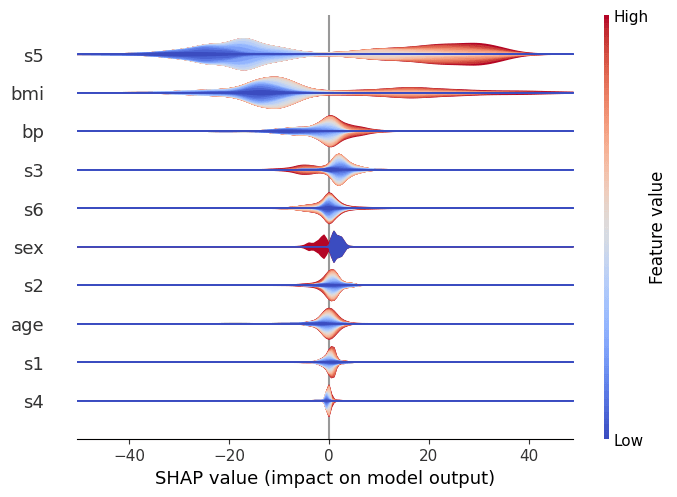
\includegraphics[width=0.45\textwidth]{figs/shap/plots/violin/example_notebooks_api_examples_plots_violin_12_0.png}
        \caption{Layered violin summary plot}
        \label{fig:layered-violin-plot}
    \end{figure}
\end{frame}

\begin{frame}{Waterfall - Plots}
    Waterfall plots are designed to display explanations for individual predictions, so they expect a single row of an Explanation object as input. The bottom of a waterfall plot starts as the expected value of the model output, and then each row shows how the positive (red) or negative (blue) contribution of each feature moves the value from the expected model output over the background dataset to the model output for this prediction.
    
    Below is an example that plots the first explanation. Note that by default \ac{SHAP} explains XGBoost classifier models in terms of their margin output, before the logistic link function. That means the units on the x-axis are log-odds units, so negative values imply probabilities of less than 0.5 that the person makes over \$50k annually. The gray text before the feature names shows the value of each feature for this sample.
\end{frame}

\begin{frame}{Waterfall - Plots}
    \begin{figure}[htbp]
        \centering
        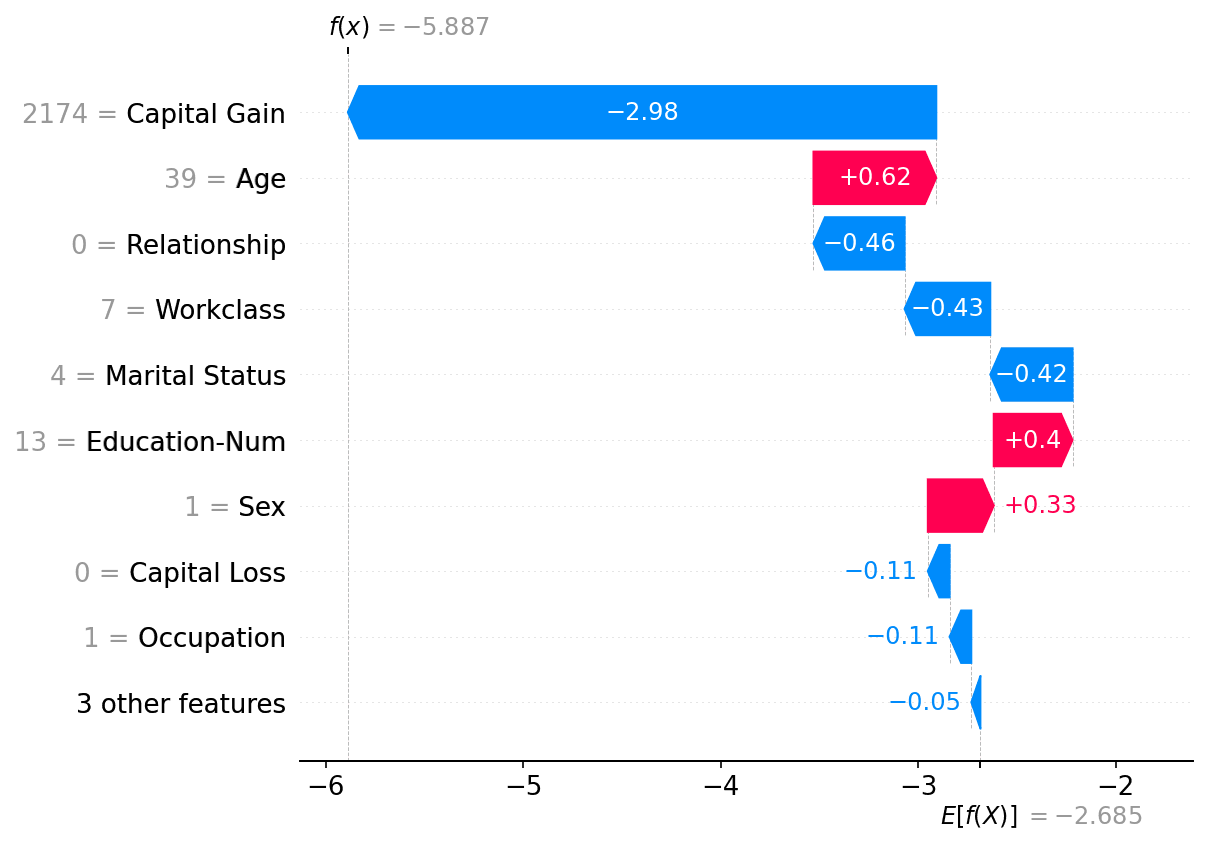
\includegraphics[width=0.65\textwidth]{figs/shap/plots/waterfall/example_notebooks_api_examples_plots_waterfall_3_0.png}
        \caption{Waterfall summary plot}
        \label{fig:waterfall-plot}
    \end{figure}
\end{frame}

\begin{frame}{Waterfall - Plots}

    It is interesting that having a capital gain of \$2,174 dramatically reduces this person’s predicted probability of making over \$50k annually. Since waterfall plots only show a single sample worth of data, we can’t see the impact of changing capital gain. To see this we can use a scatter plot, which shows how low values for capital gain are a more negative predictor of income than no capital gain at all. Why this happens would require a deeper dive into the data, and should also involve training a model more carefully and with bootstrap resamples to quantify any uncertainty in the model-building process.
\end{frame}

\begin{frame}{Waterfall - Plots}
    \begin{figure}[htbp]
        \centering
        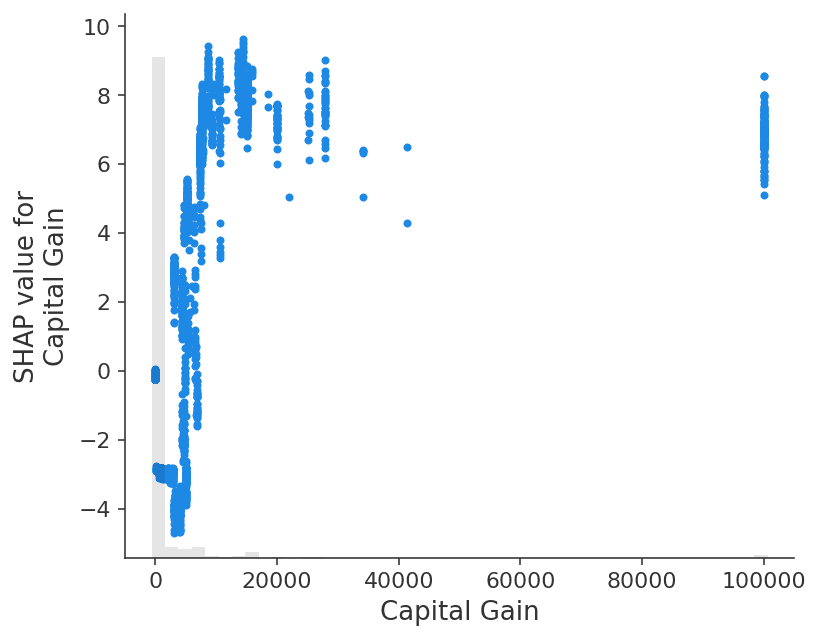
\includegraphics[width=0.6\textwidth]{figs/shap/plots/waterfall/example_notebooks_api_examples_plots_waterfall_7_0.png}
        \caption{capital gain - Waterfall summary plot}
        \label{fig:cap-waterfall-plot}
    \end{figure}
\end{frame}



\section{Project Examples}

\begin{frame}{Types - Tabular Examples}
    \begin{itemize}
        \item \textbf{Tree-based Models}
        \item \textbf{Linear Models}
        \item \textbf{Neural Networks}
        \item \textbf{Model Agnostic}
    \end{itemize}   
\end{frame}

\begin{frame}{Tree-based models - Tabular Examples}
    \begin{itemize}
        \item Basic \ac{SHAP} Interaction Value Example in XGBoost
        \item Catboost tutorial
        \item Census income classification with LightGBM
        \item Census income classification with XGBoost
        \item Example of loading a custom tree model into \ac{SHAP}
        \item Explaining a simple OR function
        \item Explaining the Loss of a Tree Model
        \item Fitting a Linear Simulation with XGBoost
        \item Force Plot Colors
        \item Front page example (XGBoost)
    \end{itemize}
\end{frame}

\begin{frame}{Tree-based models - Tabular Examples}
    \begin{itemize}
        \item League of Legends Win Prediction with XGBoost
        \item NHANES I Survival Model
        \item Speed comparison of gradient boosting libraries for shap values calculations
        \item Python Version of Tree \ac{SHAP}
        \item Scatter Density vs. Violin Plot
        \item Understanding Tree \ac{SHAP} for Simple Models
    \end{itemize}   
\end{frame}

\begin{frame}{Linear Models - Tabular Examples}
    \begin{itemize}
        \item Explaining a model that uses standardized features
        \item Math behind LinearExplainer with correlation feature perturbation
        \item Sentiment Analysis with Logistic Regression
    \end{itemize}   
\end{frame}

\begin{frame}{Neural Networks - Tabular Examples}
    \begin{itemize}
        \item Census income classification with Keras
    \end{itemize}   
\end{frame}

\begin{frame}{Model Agnostic - Tabular Examples}
    \begin{itemize}
        \item Census income classification with scikit-learn
        \item Diabetes regression with scikit-learn
        \item Iris classification with scikit-learn
        \item \ac{SHAP} Values for Multi-Output Regression Models
        \item Simple California Demo
        \item Simple Kernel \ac{SHAP}
        \item How a squashing function can affect feature importance
    \end{itemize}   
\end{frame}

\begin{frame}{Types - Text Examples}
        \begin{itemize}
        \item \textbf{Sentiment Analysis}
        \item \textbf{Translation}
        \item \textbf{Text Generation}
        \item \textbf{Summarization}
        \item \textbf{Question Answering}
        \item \textbf{Language Modelling}
        \item \textbf{Text Entailment}
    \end{itemize}
\end{frame}

\begin{frame}{Sentiment Analysis - Text Examples}
    \begin{itemize}
        \item Emotion classification multiclass example
        \item Keras LSTM for IMDB Sentiment Classification
        \item Positive vs. Negative Sentiment Classification
        \item Using custom functions and tokenizers
    \end{itemize}   
\end{frame}

\begin{frame}{Translation - Text Examples}
    \begin{itemize}
        \item Machine Translation Explanations
    \end{itemize}   
\end{frame}

\begin{frame}{Text Generation - Text Examples}
    \begin{itemize}
        \item Open Ended GPT2 Text Generation Explanations
    \end{itemize}   
\end{frame}

\begin{frame}{Summarization - Text Examples}
    \begin{itemize}
        \item Text-to-Text Explanation: Abstractive Summarization Example
    \end{itemize}   
\end{frame}

\begin{frame}{Summarization - Text Examples}
    \begin{itemize}
        \item Text-to-Text Explanation: Abstractive Summarization Example
    \end{itemize}   
\end{frame}

\begin{frame}{Question Answering - Text Examples}
    \begin{itemize}
        \item Explaining a Question Answering Transformers Model
    \end{itemize}   
\end{frame}

\begin{frame}{Language Modelling - Text Examples}
    \begin{itemize}
        \item Text to Multiclass Explanation: Language Modeling Example
    \end{itemize}   
\end{frame}

\begin{frame}{Text Entailment - Text Examples}
    \begin{itemize}
        \item Multi-Input Text Explanation: Textual Entailment with Facebook BART
    \end{itemize}
\end{frame}

\begin{frame}{Types - Image Examples}
    \begin{itemize}
        \item \textbf{Image Classification}
        \item \textbf{Image Captioning}
    \end{itemize}
\end{frame}

\begin{frame}{Image Classification - Image Examples}
    \begin{itemize}
        \item Explain PyTorch MobileNetV2 using the Partition explainer
        \item Explain ResNet50 using the Partition explainer
        \item Explain an Intermediate Layer of VGG16 on ImageNet
        \item Explain an Intermediate Layer of VGG16 on ImageNet (PyTorch)
        \item Front Page DeepExplainer MNIST Example
        \item Explain ResNet50 ImageNet classification using Partition explainer
        \item Multi-class ResNet50 on ImageNet (TensorFlow)
        \item Multi-input Gradient Explainer MNIST Example
        \item PyTorch Deep Explainer MNIST example
    \end{itemize}
\end{frame}

\begin{frame}{Image Captioning - Image Examples}
    \begin{itemize}
        \item Explaining Image Captioning (Image to Text) using Azure Cognitive Services and Partition Explainer
        \item Explaining Image Captioning (Image to Text) using Open Source Image Captioning Model and Partition Explainer
    \end{itemize}
\end{frame}

\begin{frame}{Types - Genomic Examples}
    \begin{itemize}
        \item \textbf{Compute Importance Scores}
    \end{itemize}
\end{frame}


\section{Reference}

\begin{frame}{Links - Reference}
    \begin{itemize}
        \item \textbf{Documentation:} \url{shap.readthedocs.io}
        \item \textbf{GitHub:} \url{github.com/shap/shap}
    \end{itemize}
    
\end{frame}

\section{Release Notes}

\begin{frame}{Last version - Release Notes}
    v0.43.0 - Released on 2023-10-09
\end{frame}

\section{Thank you for exploring \ac{SHAP}!}


\maketitle

\begin{frame}[allowframebreaks]{References}
\bibliographystyle{plain}
\bibliography{references}
\end{frame}

\end{document}